\documentclass{llncs}

\usepackage[utf8]{inputenc}
\usepackage{pgfplotstable}

\bibliographystyle{splncs}

\begin{document}

\title{A Polynomial-time Regular Expressions Implementation}

\author{Juan Pedro Alves Lopes \and Maria Alice Silveira de Brito \and Paulo Eustáquio Duarte Pinto}

\institute{
    Instituto de Matemática e Estatística\\  
    Universidade do Estado do Rio de Janeiro, RJ, Brazil \\
    \email{me@juanlopes.net} \email{malice@ime.uerj.br} \email{pauloedp@ime.uerj.br}
}



\maketitle

\begin{abstract}

Regular expressions are a notation to define regular languages in terms of simple composable operations. They are equivalent to finite automata in expressive power. In practice, however, modern regular expressions implementations diverge from the original theory. Most changes are made to allow greater expressive power. This convenience comes at the cost of making language membership a harder problem than it could be. In many modern languages, the regex language membership is a NP-complete problem. Besides, the way they are implemented sometimes causes expressions that could be processed in linear time to take exponential time. This fact may be seen as a security risk for many applications that use regular expressions. In this work, we suggest a simple implementation (based on Thompson's Construction Algorithm) that has superior worst-case performance than many popular implementations. We also introduce a didactic notation for automata created by this algorithm that makes the adopted implementation easier to understand.

\end{abstract}

%~~~~~~~~~~~~~~~~~~~~~~~~~~~~~~~~~~~~~~~~~~~~~~~~~~~~~~~~~~~~~~~~~~~~~~~
\section{Introduction}
%~~~~~~~~~~~~~~~~~~~~~~~~~~~~~~~~~~~~~~~~~~~~~~~~~~~~~~~~~~~~~~~~~~~~~~~

Regular expressions are a common tool in most modern languages and development platforms. Its use is widespread in the industry for many purposes, e.g. pattern recognition, extraction of tokens for formal language parsing or even user input sanitization for security purposes.

Its extensive use originates from a strong theoretical base in the finite automata field, introduced in the 40's by McCulloch and Pitts \cite{bib:McCulloch43} and formalized later by Kleene \cite{bib:Kleene56}.

Regular expressions and finite automata share a close relationship. They are equivalent in expressive power, and the conversion of the former to the latter is trivial. Ken Thompson demonstrated this in his implementation in the late 60's \cite{bib:Thompson68}, while developing the \emph{QED} text editor. The same regular expressions were later ported to the well known \emph{ed} and \emph{grep}, all part of the Unix operating system. 

Since then, as the implementations evolved, many features have been added to practical regular expressions that diverged from the original language theory. While originally regular expressions strictly describes regular languages, the currently most widespread implementation (\emph{PCRE}) is able to recognize not only any context-free language, but also some context sensitive ones. \cite{bib:Nikita12}.

One of the most notable consequences of this evolution consists in the recognition of language strings described by those expressions, a problem with linear solution originally, having exponential solutions in a large number of modern implementations, including several of the mostly used ones. Perhaps the most dangerous feature in this regard are the \emph{backreferences}, that makes membership a NP-complete problem \cite{bib:Campeanu07}. However, even expressions that could be recognized with finite automata, due to some particularities of implementation, may take exponential time in the worst case \cite{bib:Cox07}.

Languages like Python, Java and Ruby are widely used in industry, but their standard libraries implement vulnerable regular expressions. These implementations make the use of regular expressions potentially unsafe in otherwise trivial situations. A malicious user may be able to force the execution of an expression with exponential time to perform a denial-of-service attack on a web server.

For example, allowing user input to be interpreted as regular expressions, a malicious user could inject the expression $(a|a)^+b$, which given its exponential complexity in vulnerable implementations, would use 100\% of CPU for a virtually infinite time if matched against the string $aaa...aaa$. Such attacks may cause instability and unavailability of the web service. 

The prevention of this type of attack is often not trivial, as in the case of Java, where commonly used methods, such as \emph{replaceAll} and \emph{split} -- of the class \emph{String} -- are implemented with regular expressions which are vulnerable to this kind of attack. 

Even in cases where a malicious user does not have access to write regular expressions, a programming error can leave the system vulnerable to DoS attacks. This problem becomes critical with the frequent sharing of regexes in online repositories that contain many vulnerable expressions \cite{bib:Kirrage13,bib:Weidman10}. 

This work has two main objectives. The first is to demonstrate through tests and benchmarks the fundamental problems in implementations of regular expressions in several modern languages. The second objective is to achieve a didactic and minimalist implementation of regular expressions, using the theory described by Kleene and the method proposed by Thompson to construct and simulate the automaton.

The implementation proposed in this work does not include certain features which are common most modern \emph{flavors} of regular expressions. Some of these features can be implemented without sacrificing execution efficiency; whereas others may introduce some complexity, while still running in polynomial time. Some features, however, can not be implemented without making the algorithm exponential in the worst case.

We intend to show in this paper that the problem of recognizing strings in the languages denoted by regular expressions can be efficiently solved even with the simplest implementations, provided that its theory is observed.

%~~~~~~~~~~~~~~~~~~~~~~~~~~~~~~~~~~~~~~~~~~~~~~~~~~~~~~~~~~~~~~~~~~~~~~~
\section{Automaton Construction and Simulation}
%~~~~~~~~~~~~~~~~~~~~~~~~~~~~~~~~~~~~~~~~~~~~~~~~~~~~~~~~~~~~~~~~~~~~~~~

Given the synergy between regular expressions and finite automata and considering the ease of dealing with each of them in specific situations, it is useful to be able to convert between them. Ken Thompson \cite{bib:Thompson68} described a method for constructing automata from regular expressions. 

The method consists in building the automaton recursively by analyzing the syntax tree of the expression, a procedure that needs to be done before start to build the automaton. In the original paper by Thompson, this step was done by building the expression in \emph{infix} notation. However, in order to allow extensibility of expression format, we will define the full grammar of regular expressions that are accepted.

\subsection{Syntactic Analysis}

The first step in the construction of the automaton is to parse the expression, building the abstract syntax tree. A simple generative grammar can be defined -- using the EBNF (\emph{Extended Backus-Naur Form}) -- that represents the language formed by all regular expressions.


\begin{verbatim}
<option>     ::= <sequence> { "|" <sequence> }*
<sequence>   ::= <repetition> { <repetition> }*
<repetition> ::= <primary> { "*" | "?" | "+" }*
<primary>    ::= "." | <literal> | "(" <option> ")"
\end{verbatim}

It is not defined, but \texttt{<literal>} is any character except any of \texttt{.*?+|()}. 

In this way, the expression can be easily analyzed. For example, the expression $(a|a)^+$ b would be evaluated as the tree depicted in Figure~\ref{fig:aab_parse_tree}.

\begin{figure}[!htbp]
  \centering
  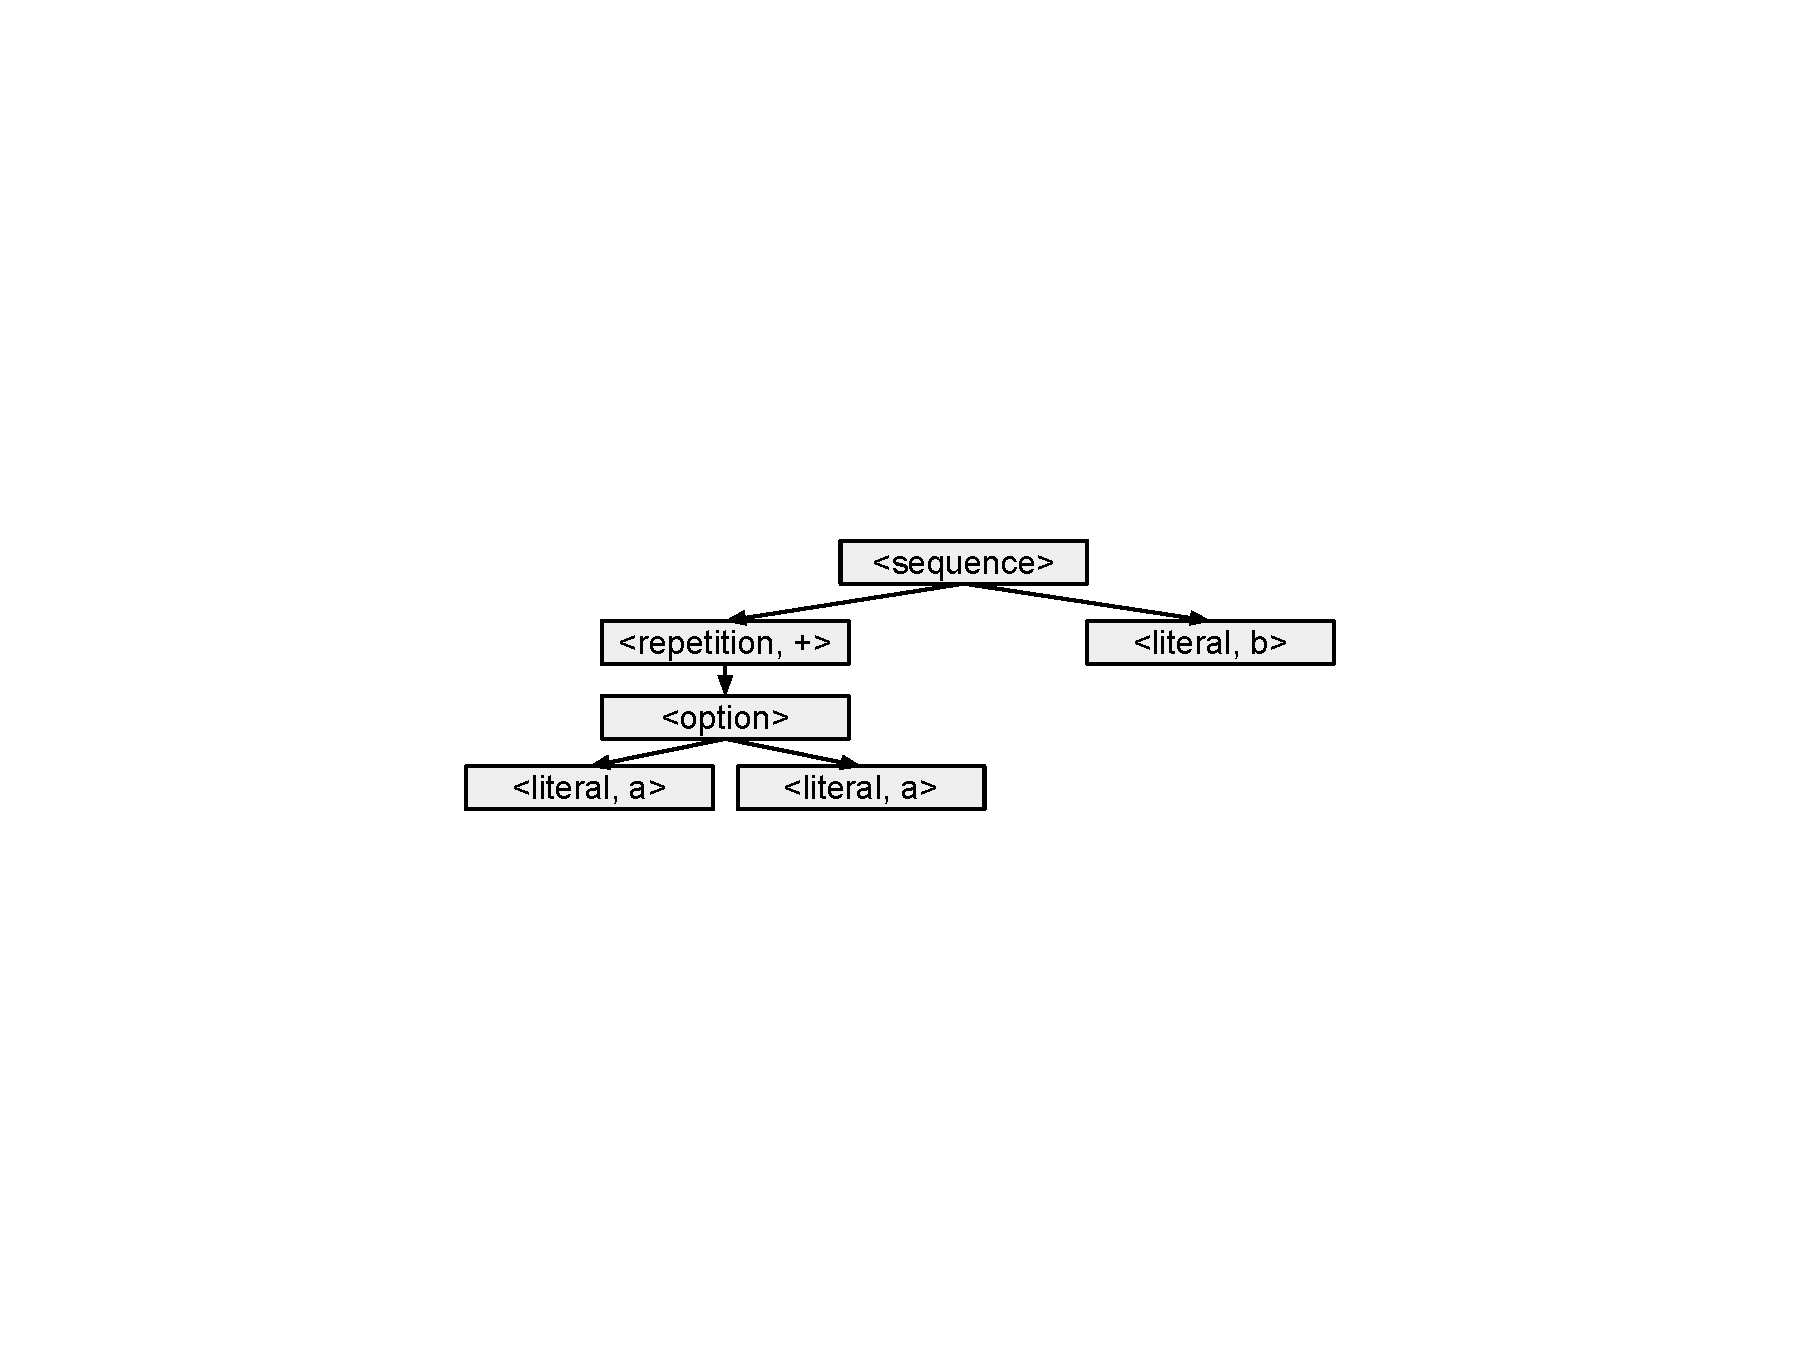
\includegraphics[trim=3.7in 3.7in 3.7in 3.7in, scale=0.50]{figures/aab_parse_tree.pdf}
  \caption{AST for the expression $(a|a)^+b$. In this case, we omit the trivial nodes, e.g. \emph{option} nodes with a single \emph{sequence} inside, \emph{repetition} nodes without any repetition operator, etc.}
  \label{fig:aab_parse_tree}
\end{figure}

Using the EBNF, the tree can be produced by several parser generator tools present in many languages. Notable examples include the YACC (\emph{Yet Another Compiler Compiler}), the JavaCC (\emph{Java Compiler Compiler}) and ANTLR (\emph{ANother Tool for Language Recognition}). 

With this AST, conversion to finite automaton becomes rather trivial, as will be discussed in the next sections.

\subsection{Notation}\label{sec:Notacao}

We will introduce an unusual notation to represent the automaton, that will make the construction easier. For convenience purposes, every state $q_i \in Q$ will be of one of three possible types:

\begin{enumerate}
    \item {\sc Consume} state: has as single transition that consumes a single character from the input;
    \item {\sc Jump} state: has one or more $\epsilon$ transitions to distinct states;
    \item {\sc Match} state: an accept state with no transitions.
\end{enumerate}

Figure~\ref{fig:nova_notacao} shows how the states in this notation may be represented in a diagram.

\begin{figure}[!htbp]
  \centering
  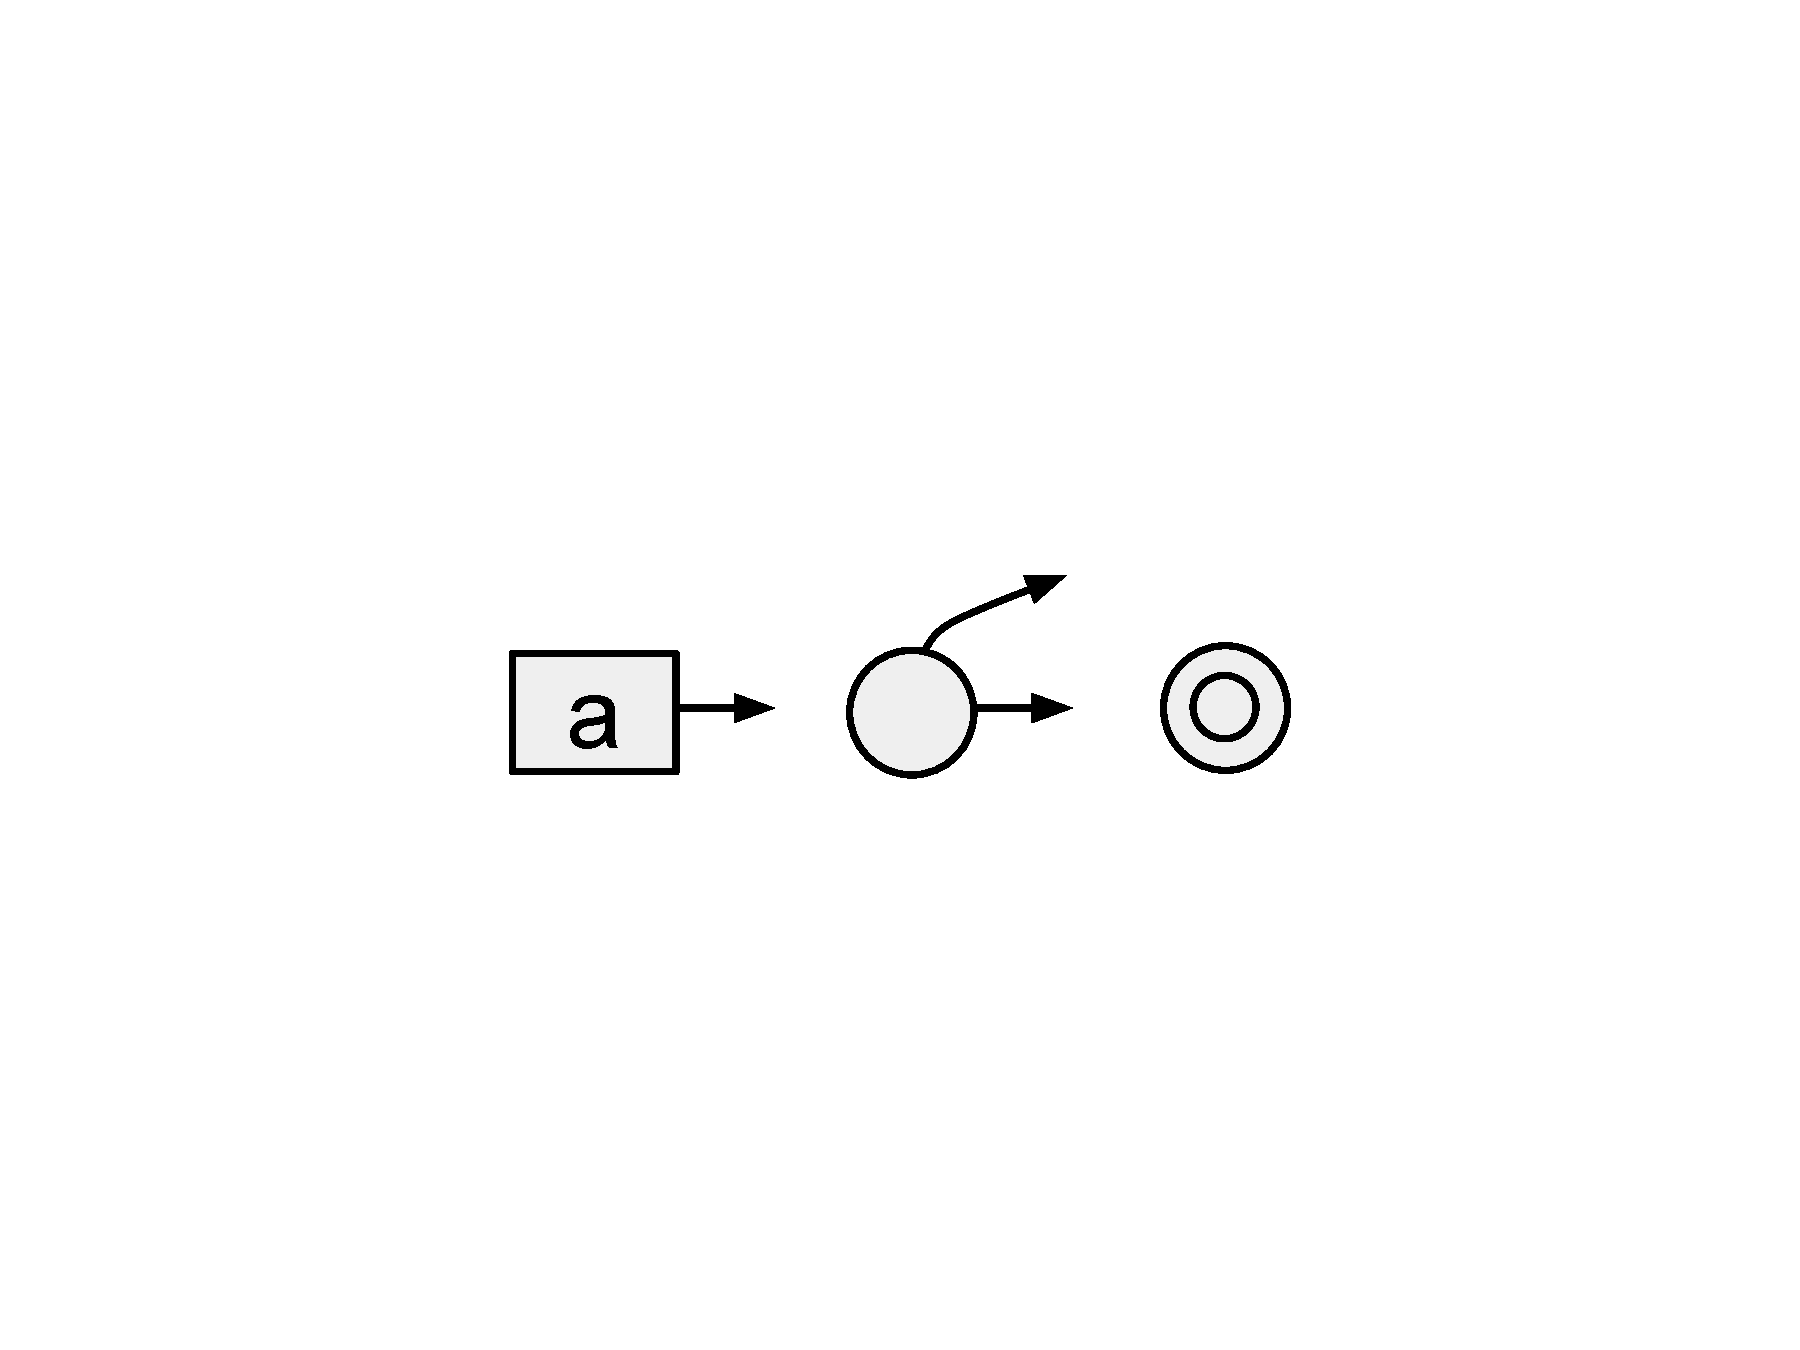
\includegraphics[trim=4in 4in 4in 4in, scale=0.30]{figures/new_notation.pdf}
  \caption{Example state representation in the new notation}
  \label{fig:nova_notacao}
\end{figure}

This representation simplifies visualization by omitting the $\epsilon$ transitions and emphasizing the difference between the {\sc Consume} and {\sc Jump} states. An example state diagram in the new notation can be seen in Figure~\ref{fig:exemplo_nova_notacao}.

\begin{figure}[!htbp]
  \centering
  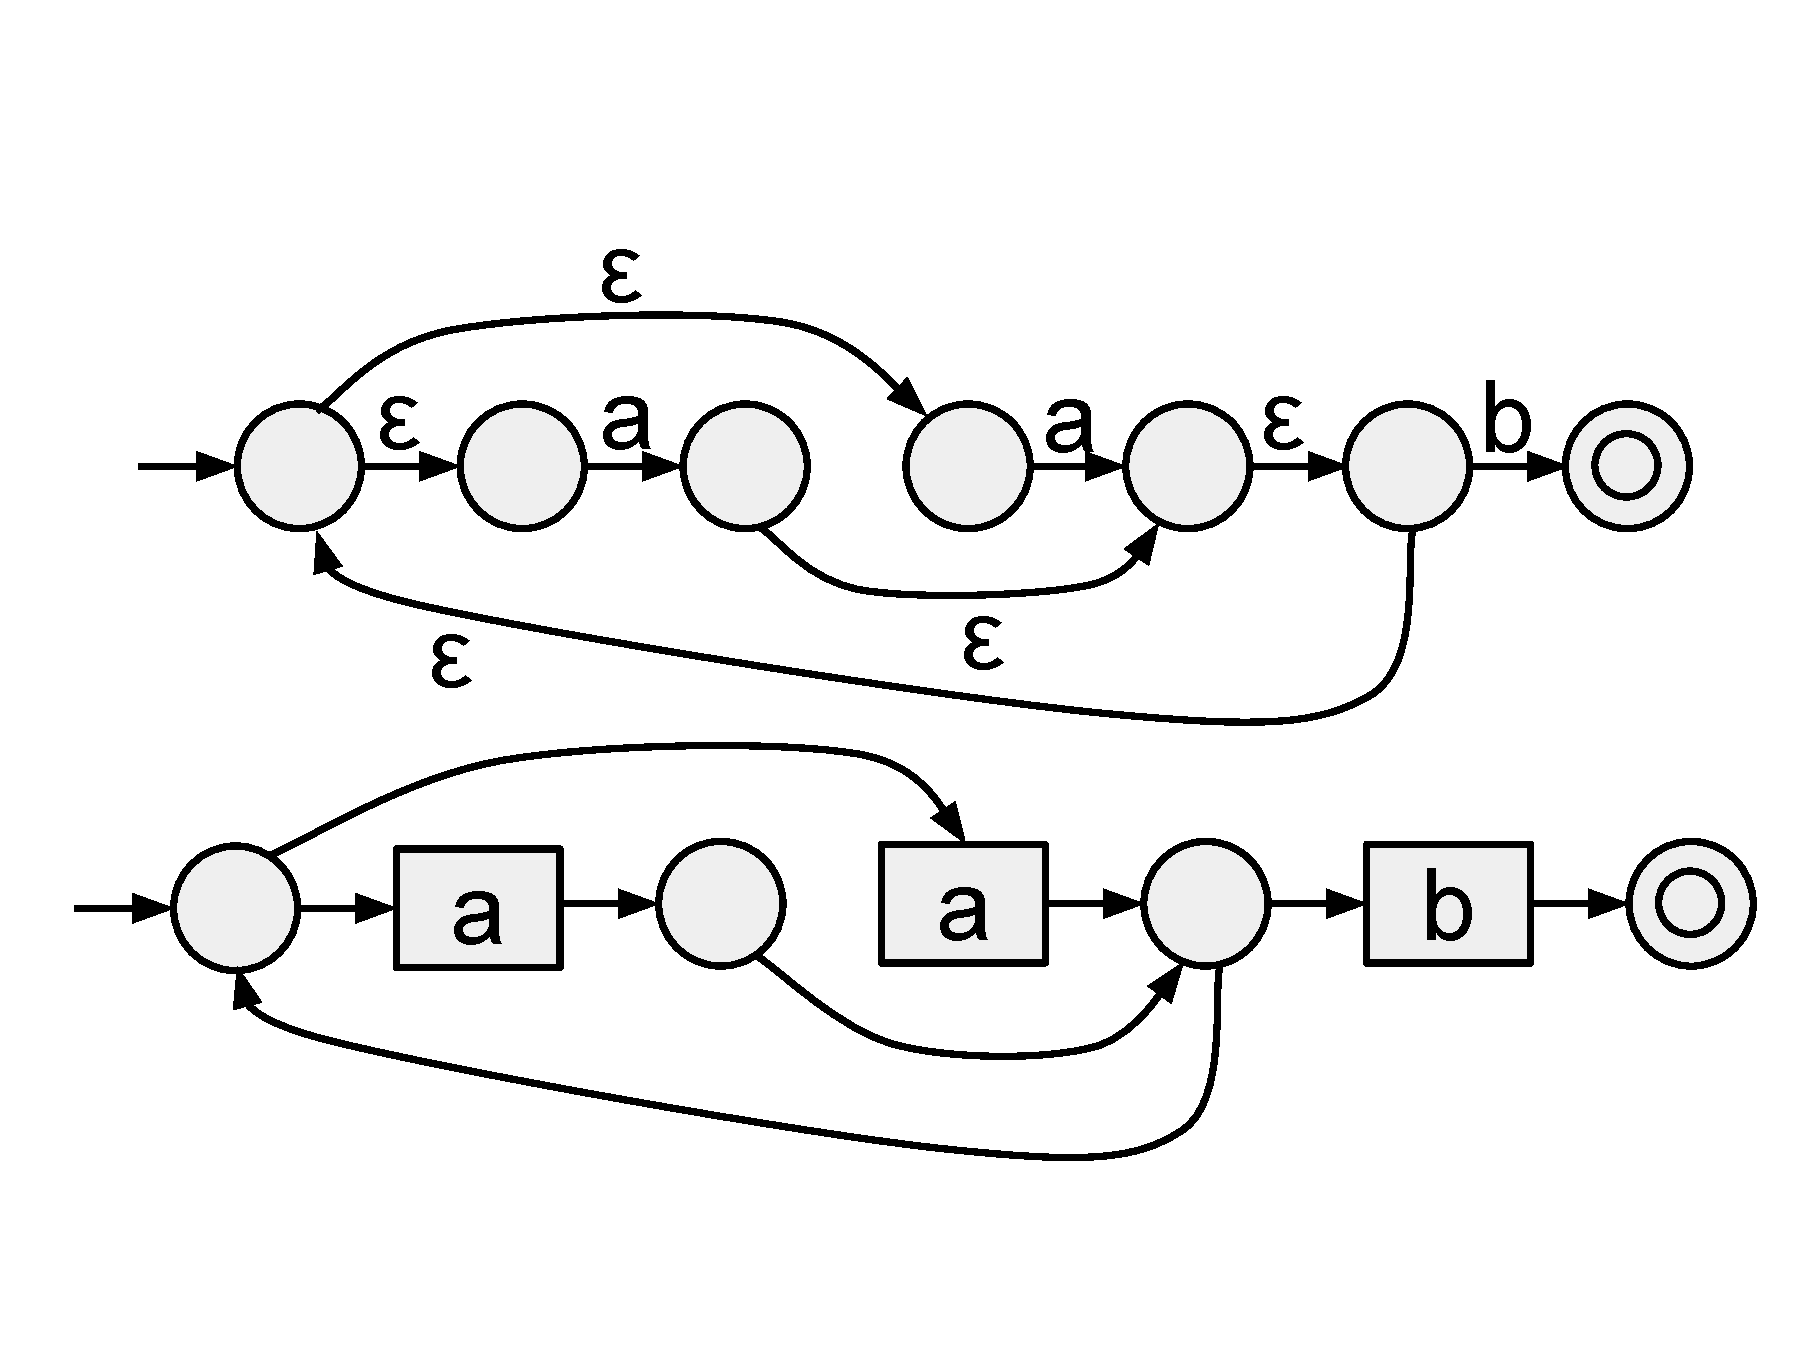
\includegraphics[trim=2in 2in 2in 2in, scale=0.25]{figures/new_notation_example.pdf}
  \caption{Same automaton represented in both ways}
  \label{fig:exemplo_nova_notacao}
\end{figure}

The diagram in Figure~\ref{fig:exemplo_nova_notacao} denotes the regular expression $(a|a)+b$. The sequential disposition of the states has some advantages, as it allows direct translation to a program-like representation (as a series of instructions). This automaton, for instance, can be translated as:

\nopagebreak 
\begin{verbatim}
0000: JUMP (+1, +3)
0001: CONSUME a
0002: JUMP (+2,)
0003: CONSUME a
0004: JUMP (+1, -4)
0005: CONSUME b
0006: MATCH!
\end{verbatim}

The {\sc Jump} instructions with more than one label express the non-determinism of the automaton. If a deterministic machine was built to run these instructions, when faced with {\sc Jump}s it could proceed to any of the defined addresses.

\subsection{Construction}

The construction of the automaton consists in recursively converting each of the nodes in the AST to a specific automaton following a recipe. Each of these recipes has only one input state and all transitions that do not point to a node within the automaton itself, point to a single output node. 

The following table shows the conversion for each node type. For notational purposes, capital letters represent complex automata produced with inner nodes, but they all follow the same construction rule.

\begin{table}
\begin{center}
	\caption{Automaton construction for each expression type}
	\begin{tabular}{ >{\centering\arraybackslash}m{0.6in} | >{\centering\arraybackslash}m{0.7in} | >{\centering\arraybackslash}m{1.3in} | m{1.8in} }

		\hline
		{\bf Type} & {\bf Expression} & {\bf Construction} & \centering\arraybackslash{\bf Instructions} \\
		\hline
		Literal & $a$ & 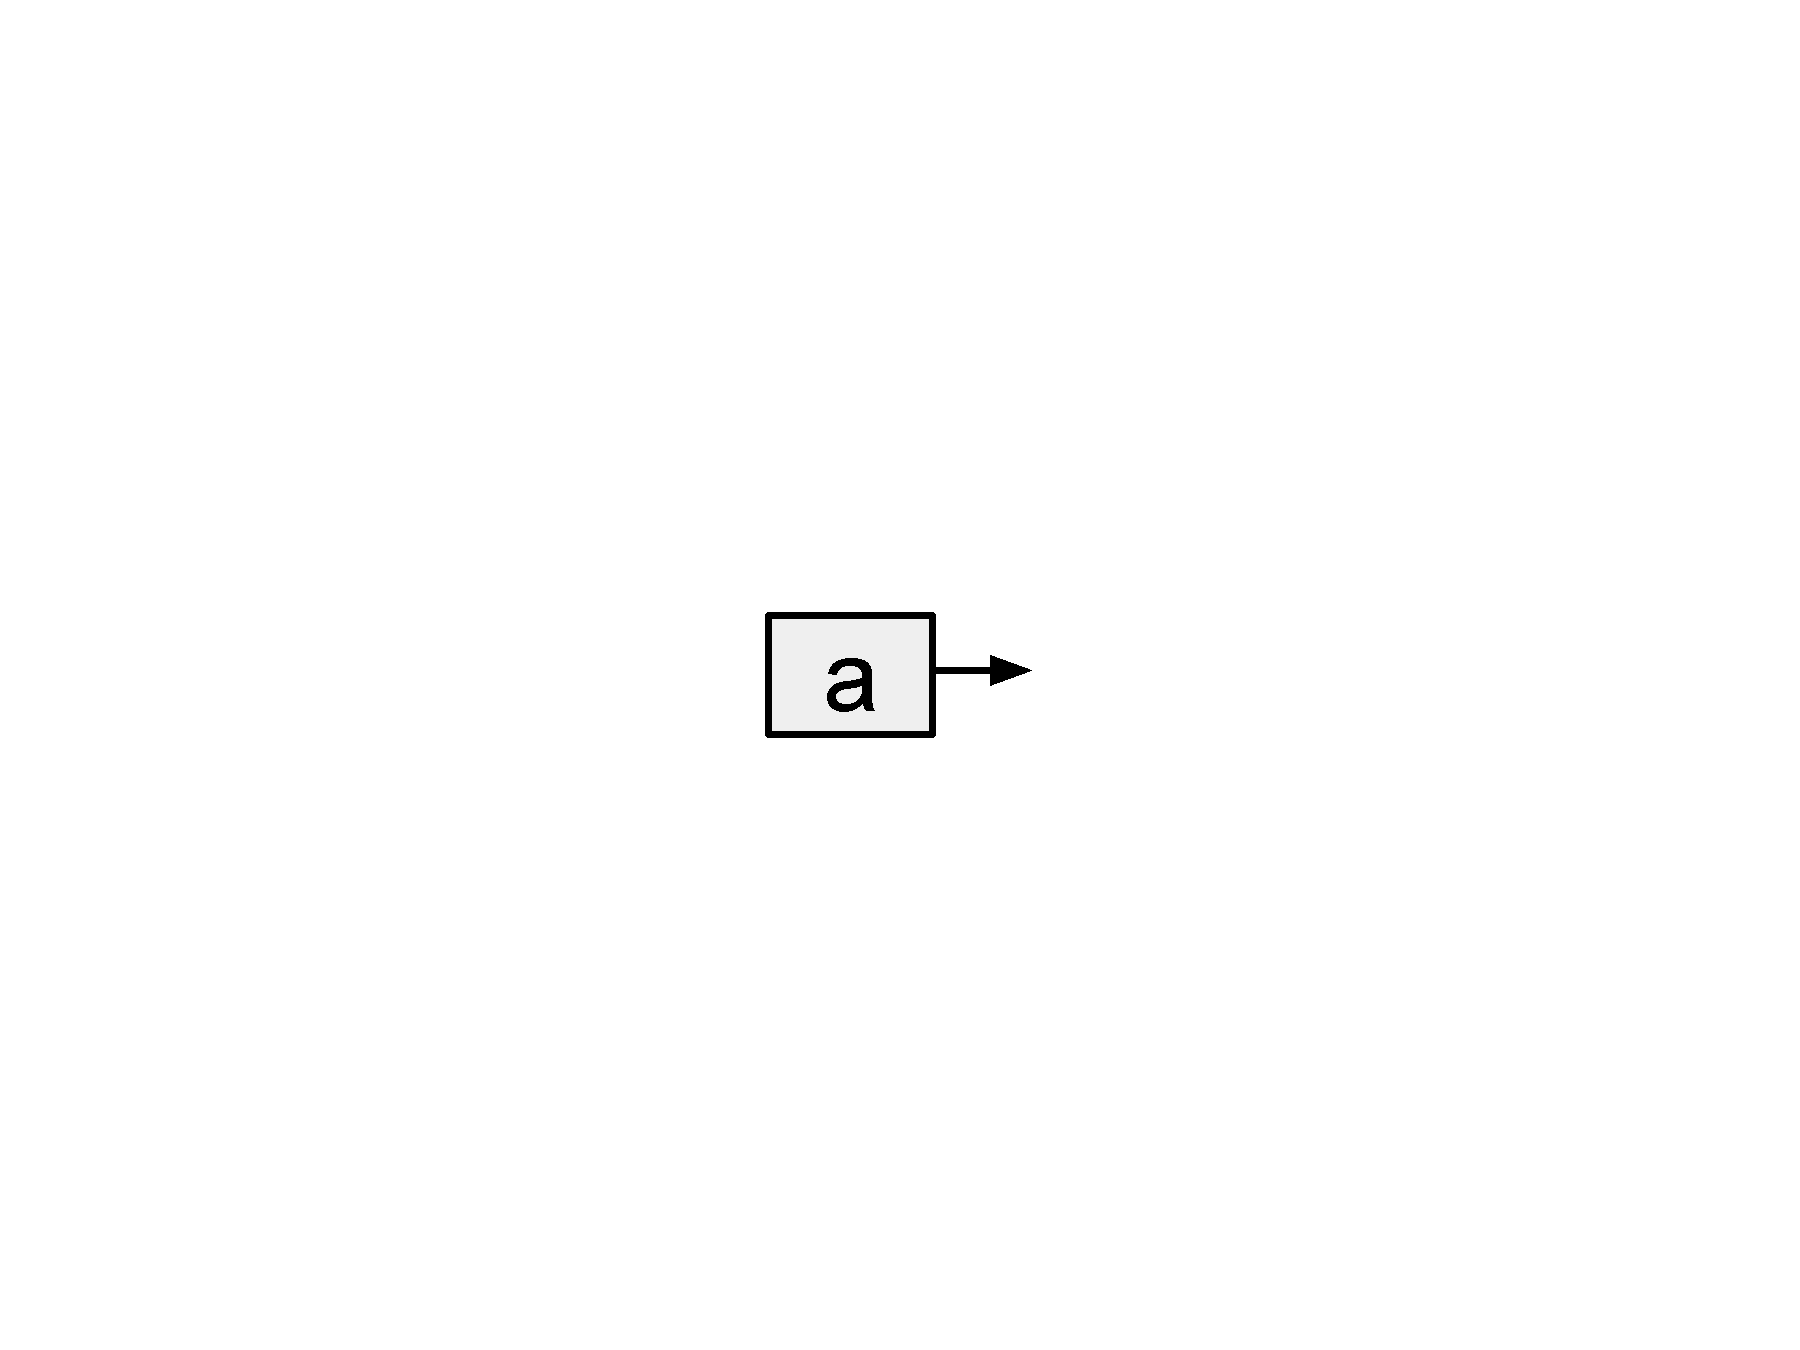
\includegraphics[trim=4in 4in 4in 3.8in, scale=0.20]{figures/thompson_literal.pdf} &
            \texttt{CONSUME a}
        \\

		\hline
		Sequence & $ST$ & 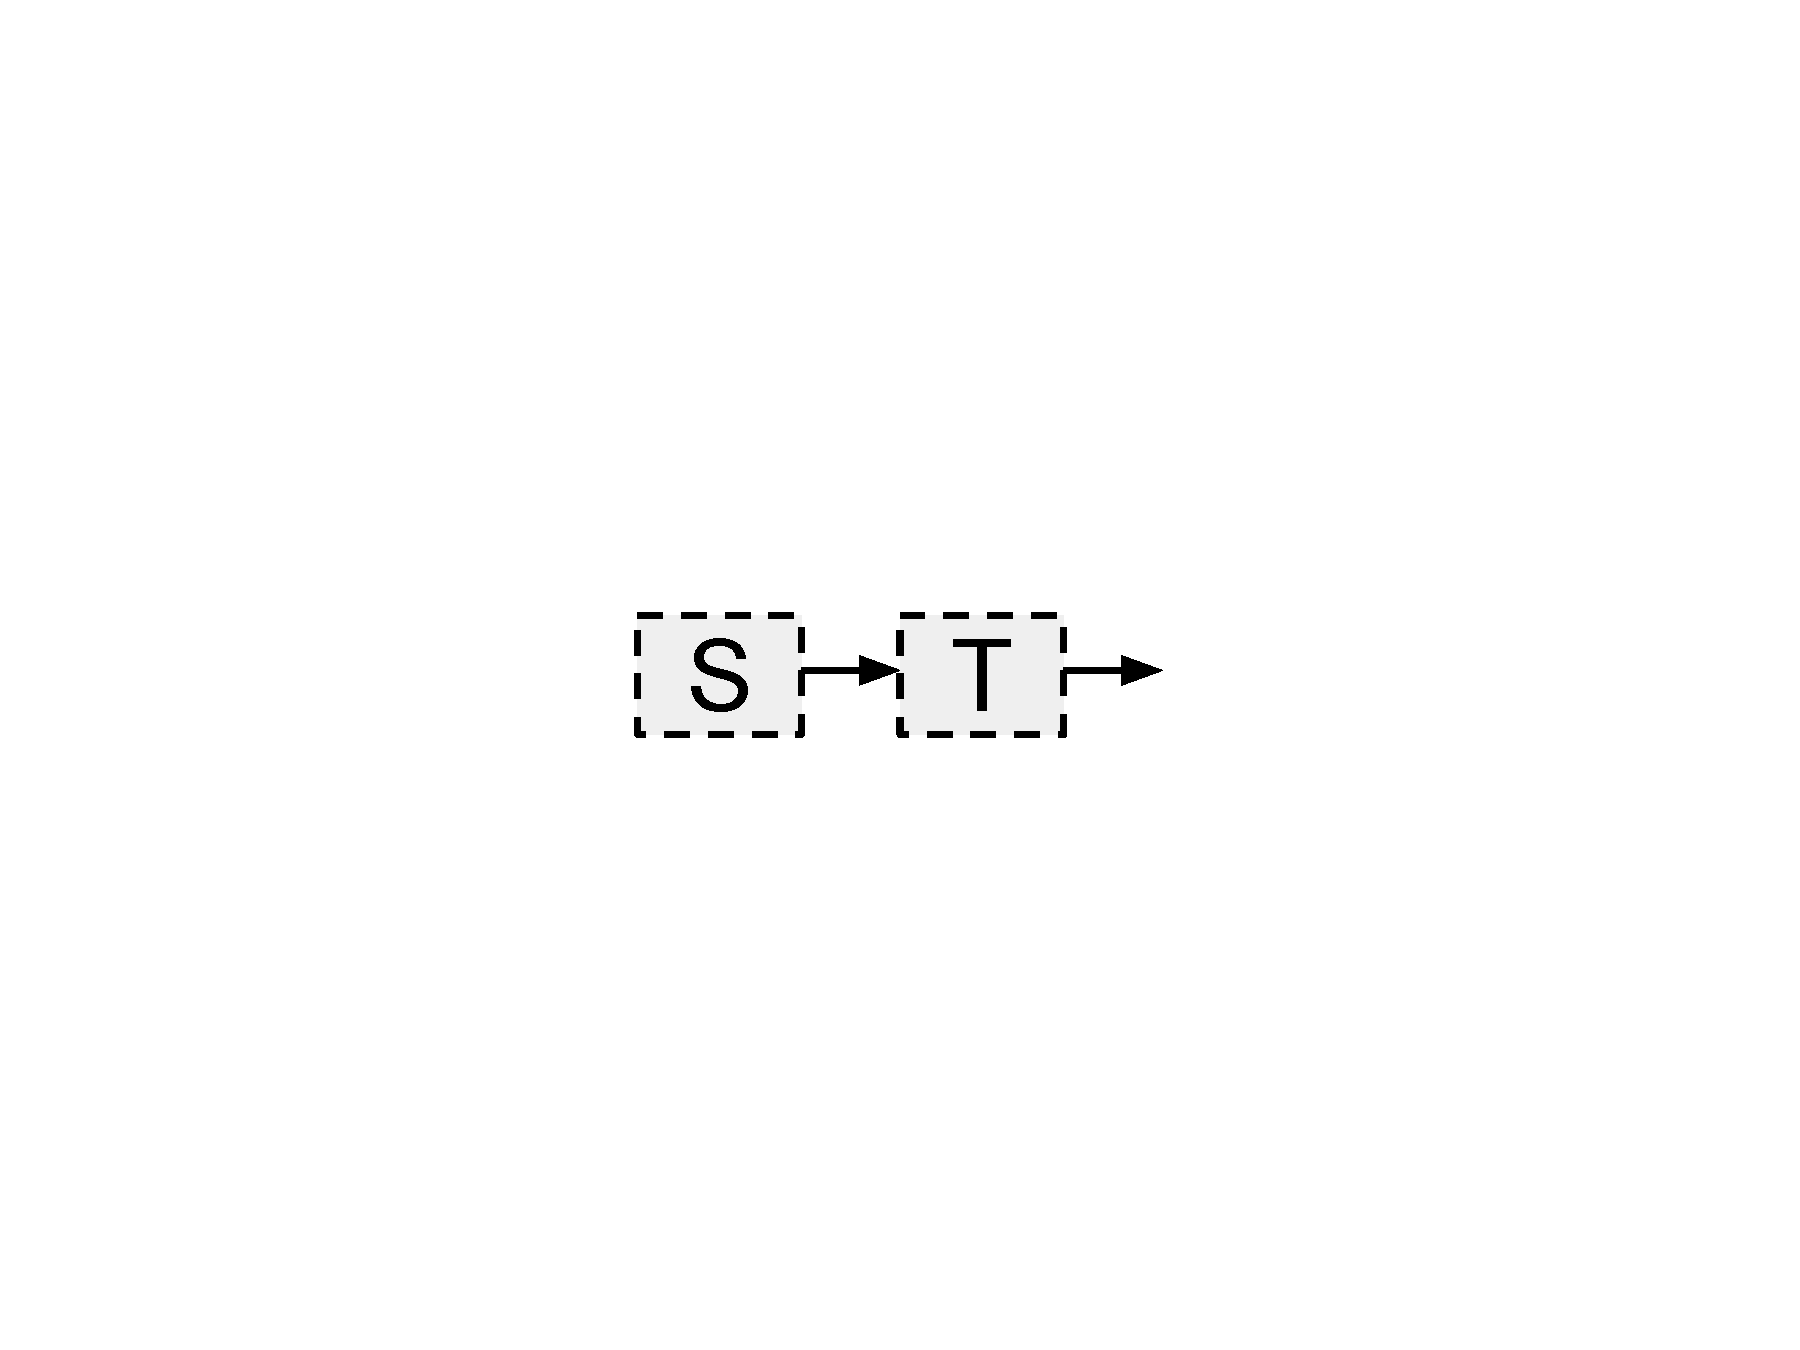
\includegraphics[trim=4in 4in 4in 3.8in, scale=0.20]{figures/thompson_sequence.pdf} &
            \texttt{<instructions of S>} \newline
            \texttt{<instructions of T>}
        \\
		\hline
		Option & $S|T$ & 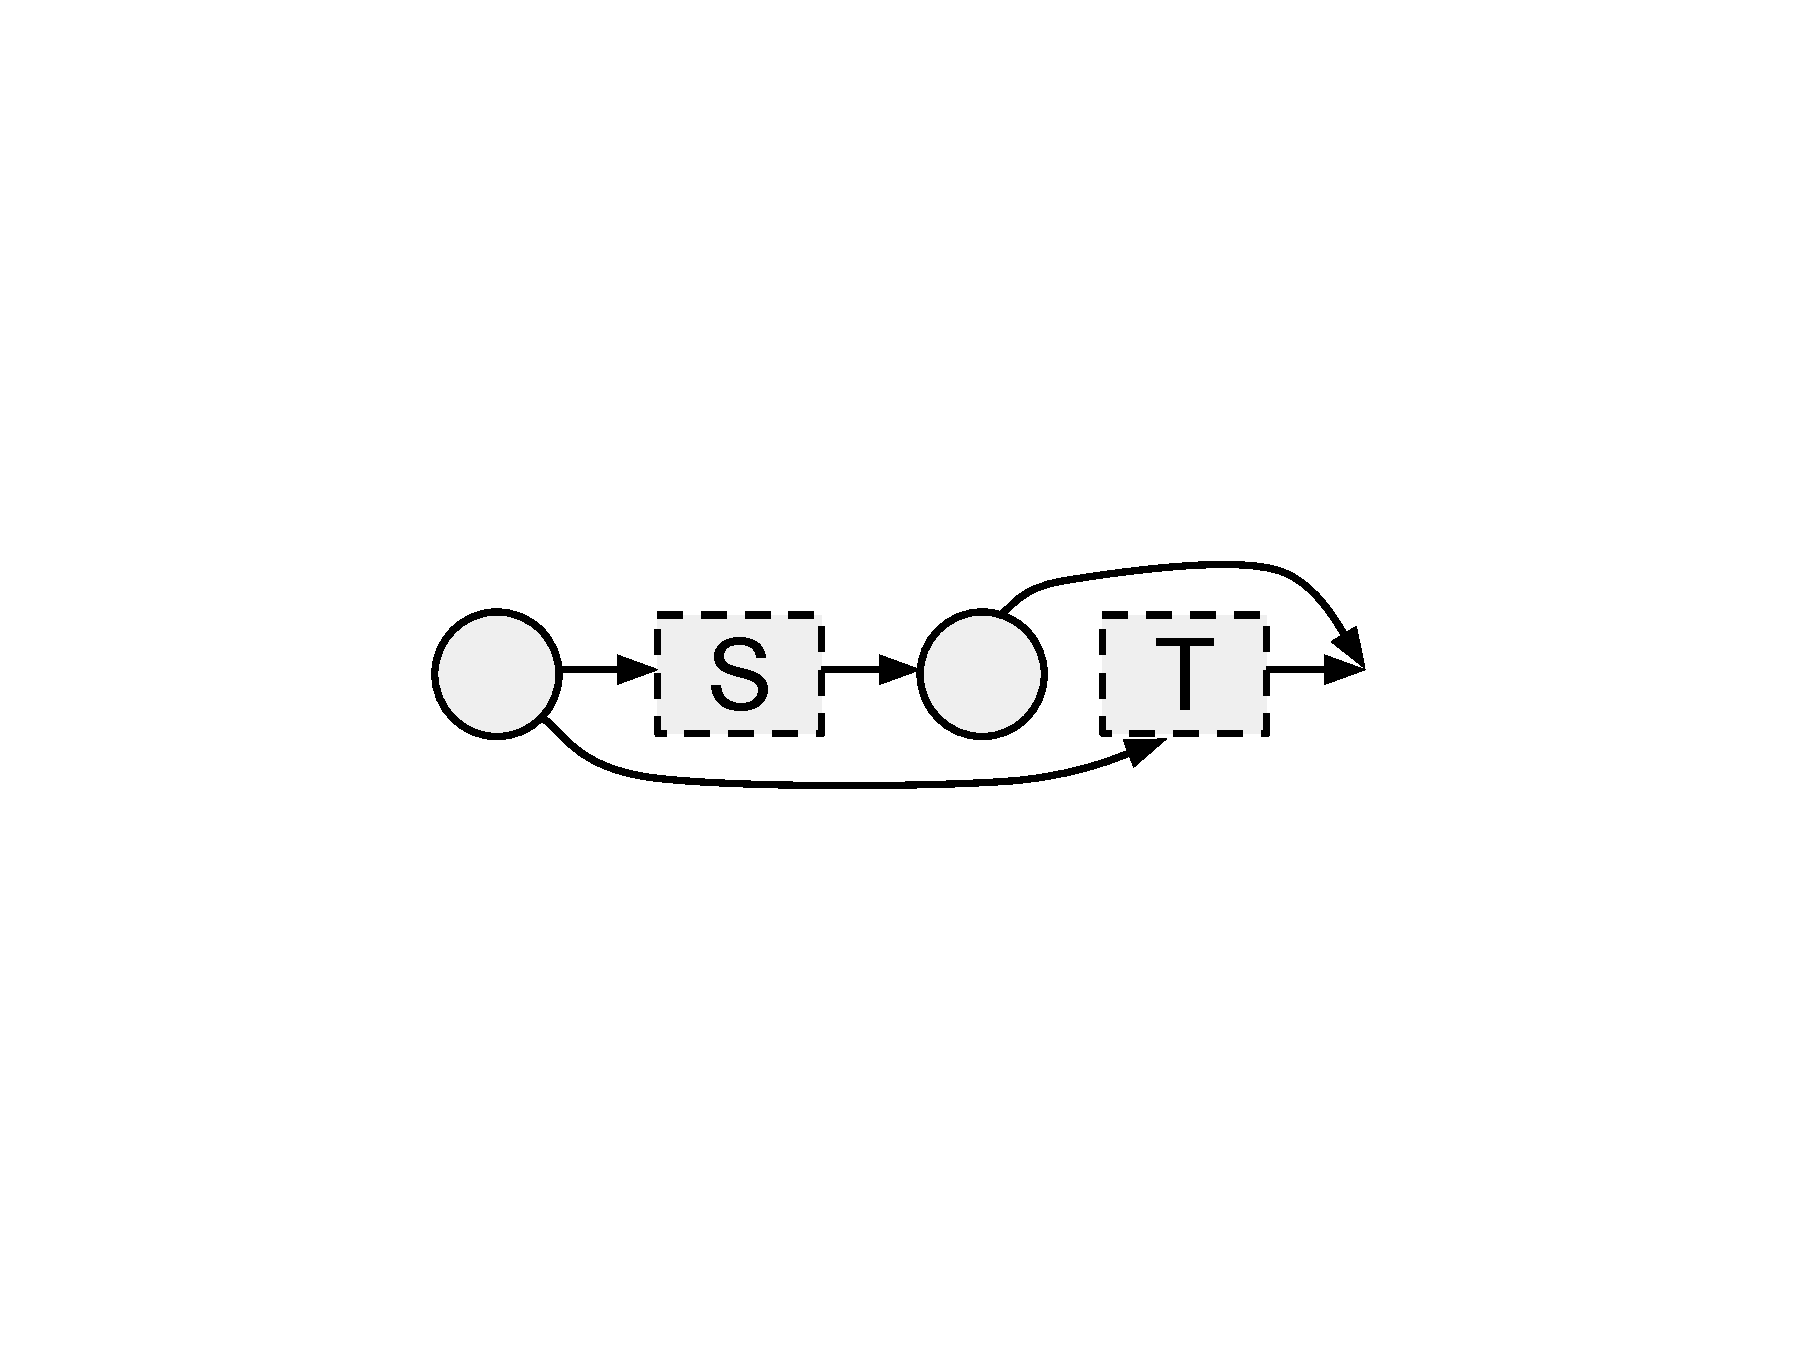
\includegraphics[trim=4in 3.7in 4in 3.5in, scale=0.20]{figures/thompson_option.pdf} &
            \texttt{JUMP (+1, <size of S>+2)} \newline
            \texttt{<instructions of S>} \newline
            \texttt{JUMP (<size of T>+1)} \newline
            \texttt{<instructions of T>}
        \\
		\hline
		Kleene+ & $S+$ & 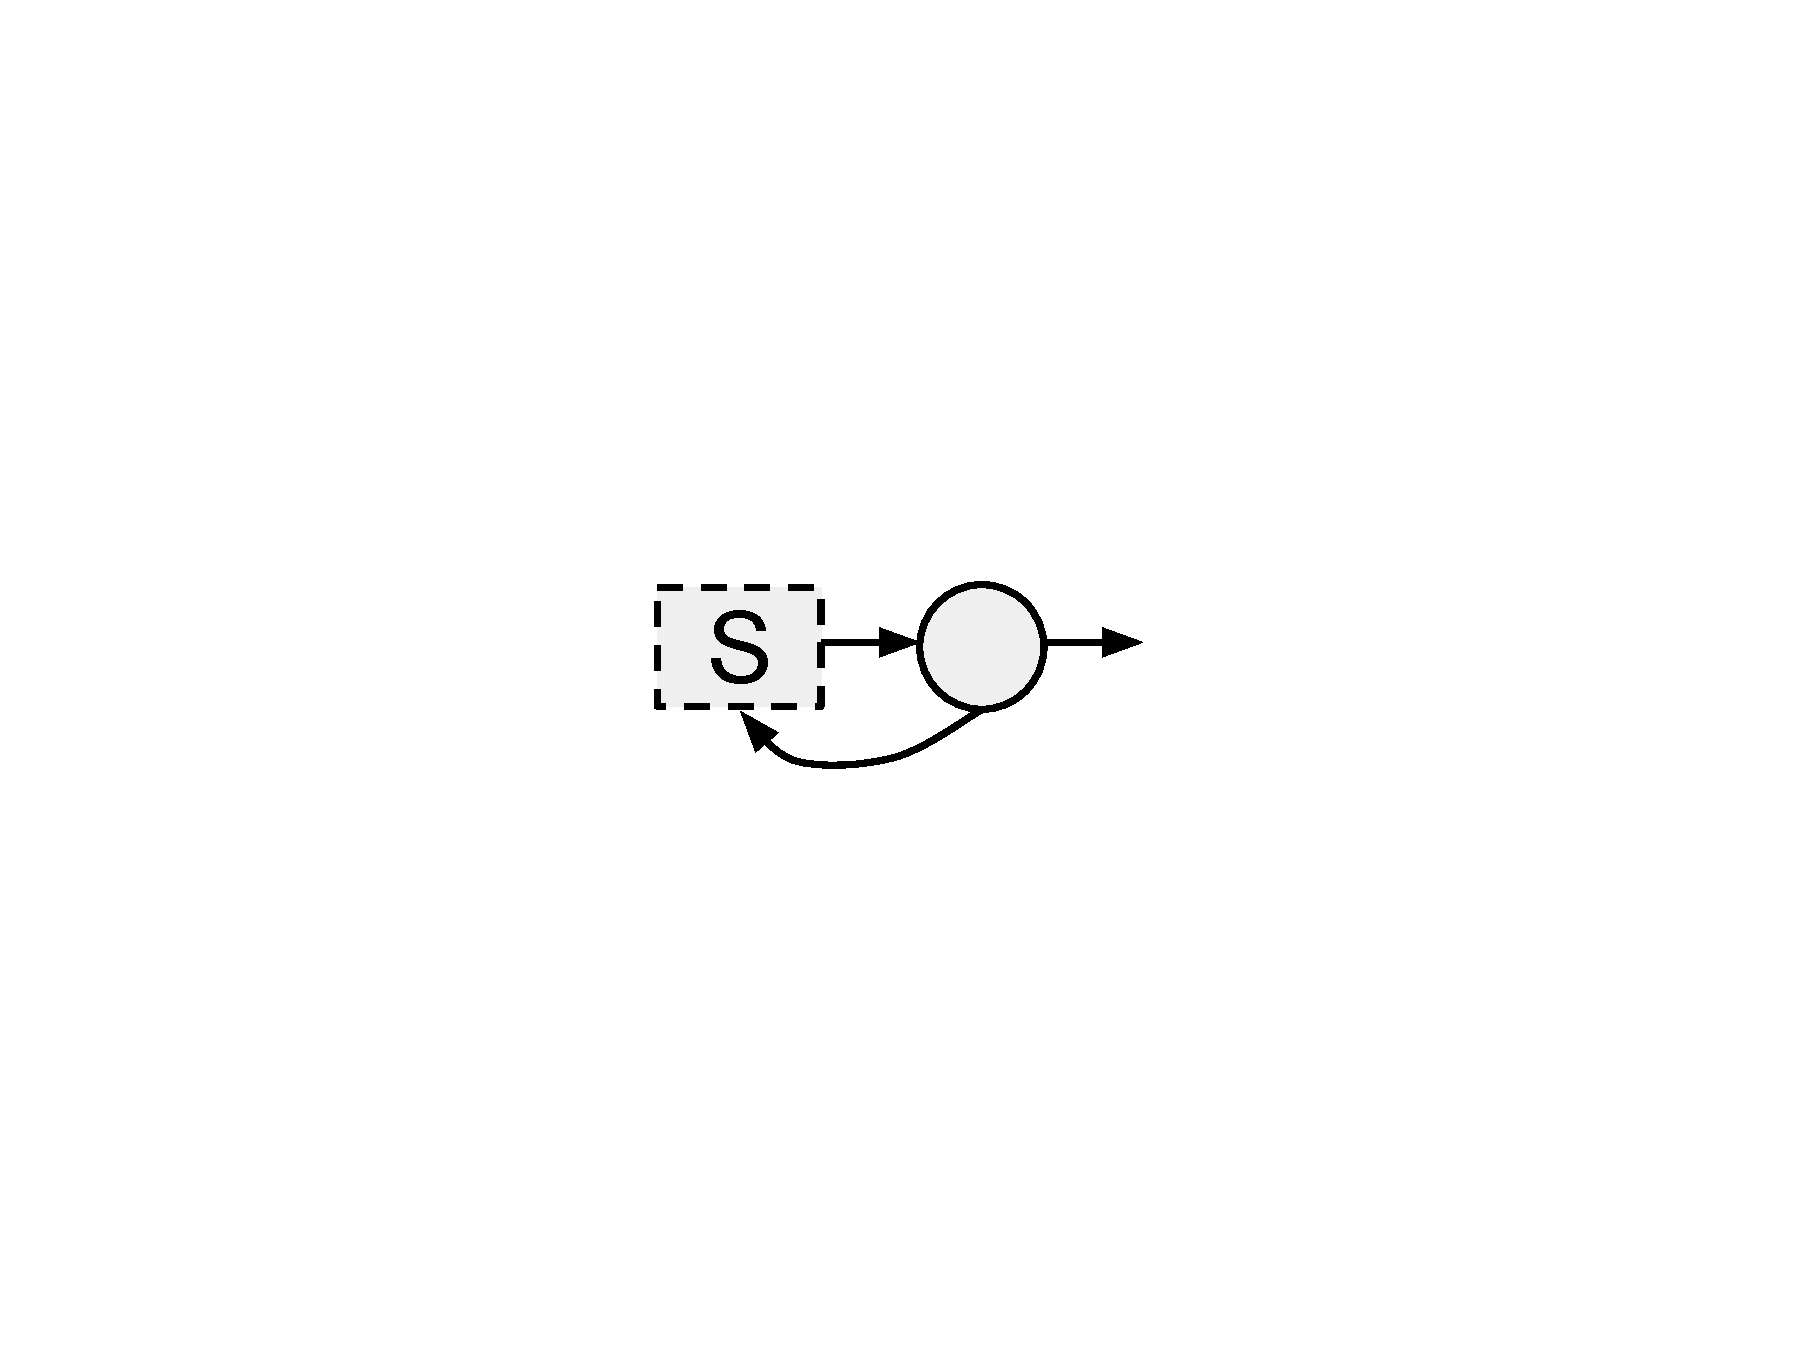
\includegraphics[trim=4in 3.7in 4in 3.5in, scale=0.20]{figures/thompson_plus.pdf} &
            \texttt{<instructions of S>} \newline
            \texttt{JUMP (+1, -<size of S>)}
        \\
		\hline
		Optional & $S?$ & 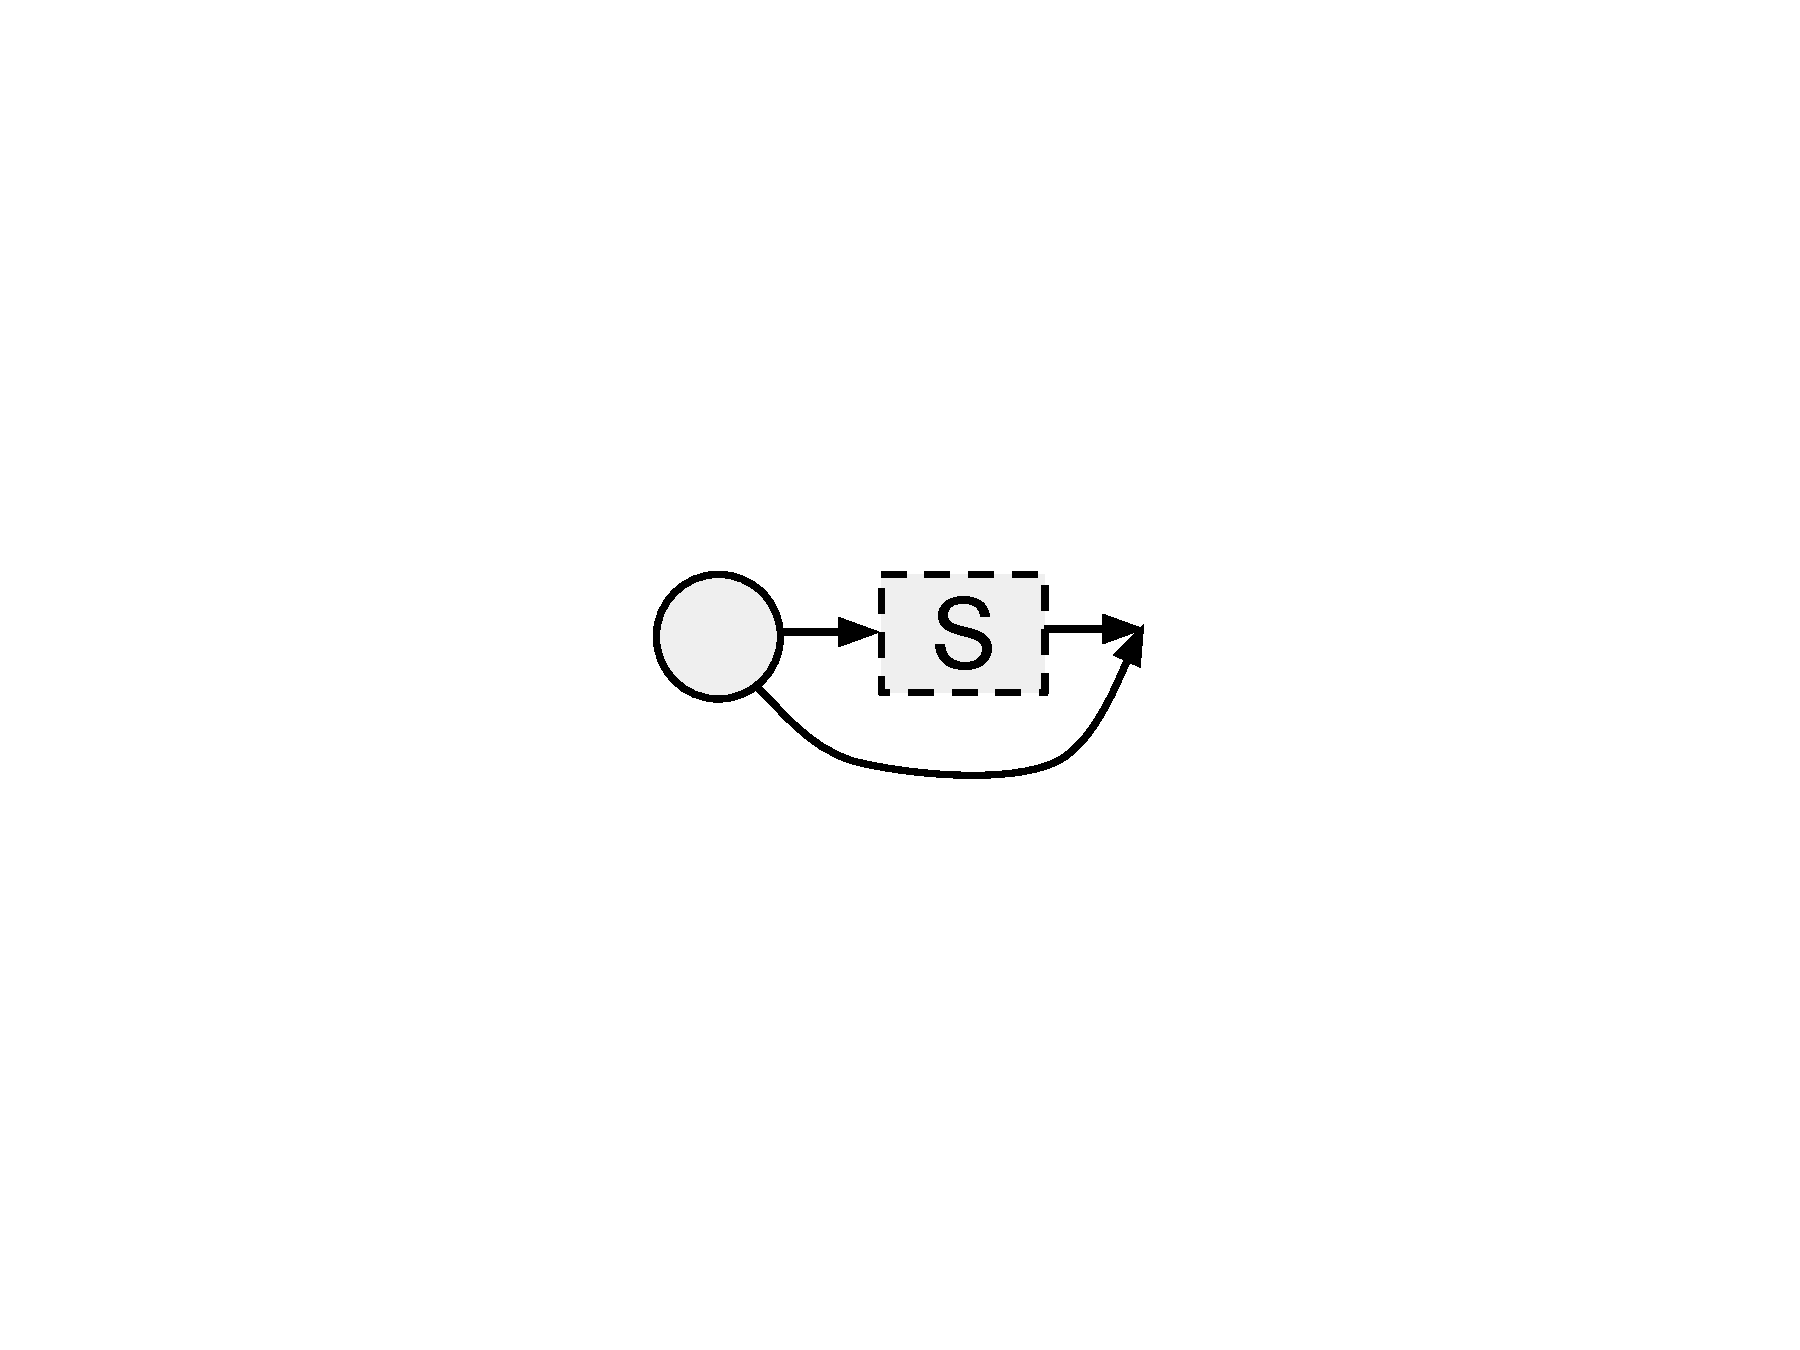
\includegraphics[trim=4in 3.7in 4in 3.5in, scale=0.20]{figures/thompson_question.pdf} &
            \texttt{JUMP (+1, <size of S>+1)} \newline
            \texttt{<instructions of S>}
        \\
		\hline
		Kleene* & $S*$ & 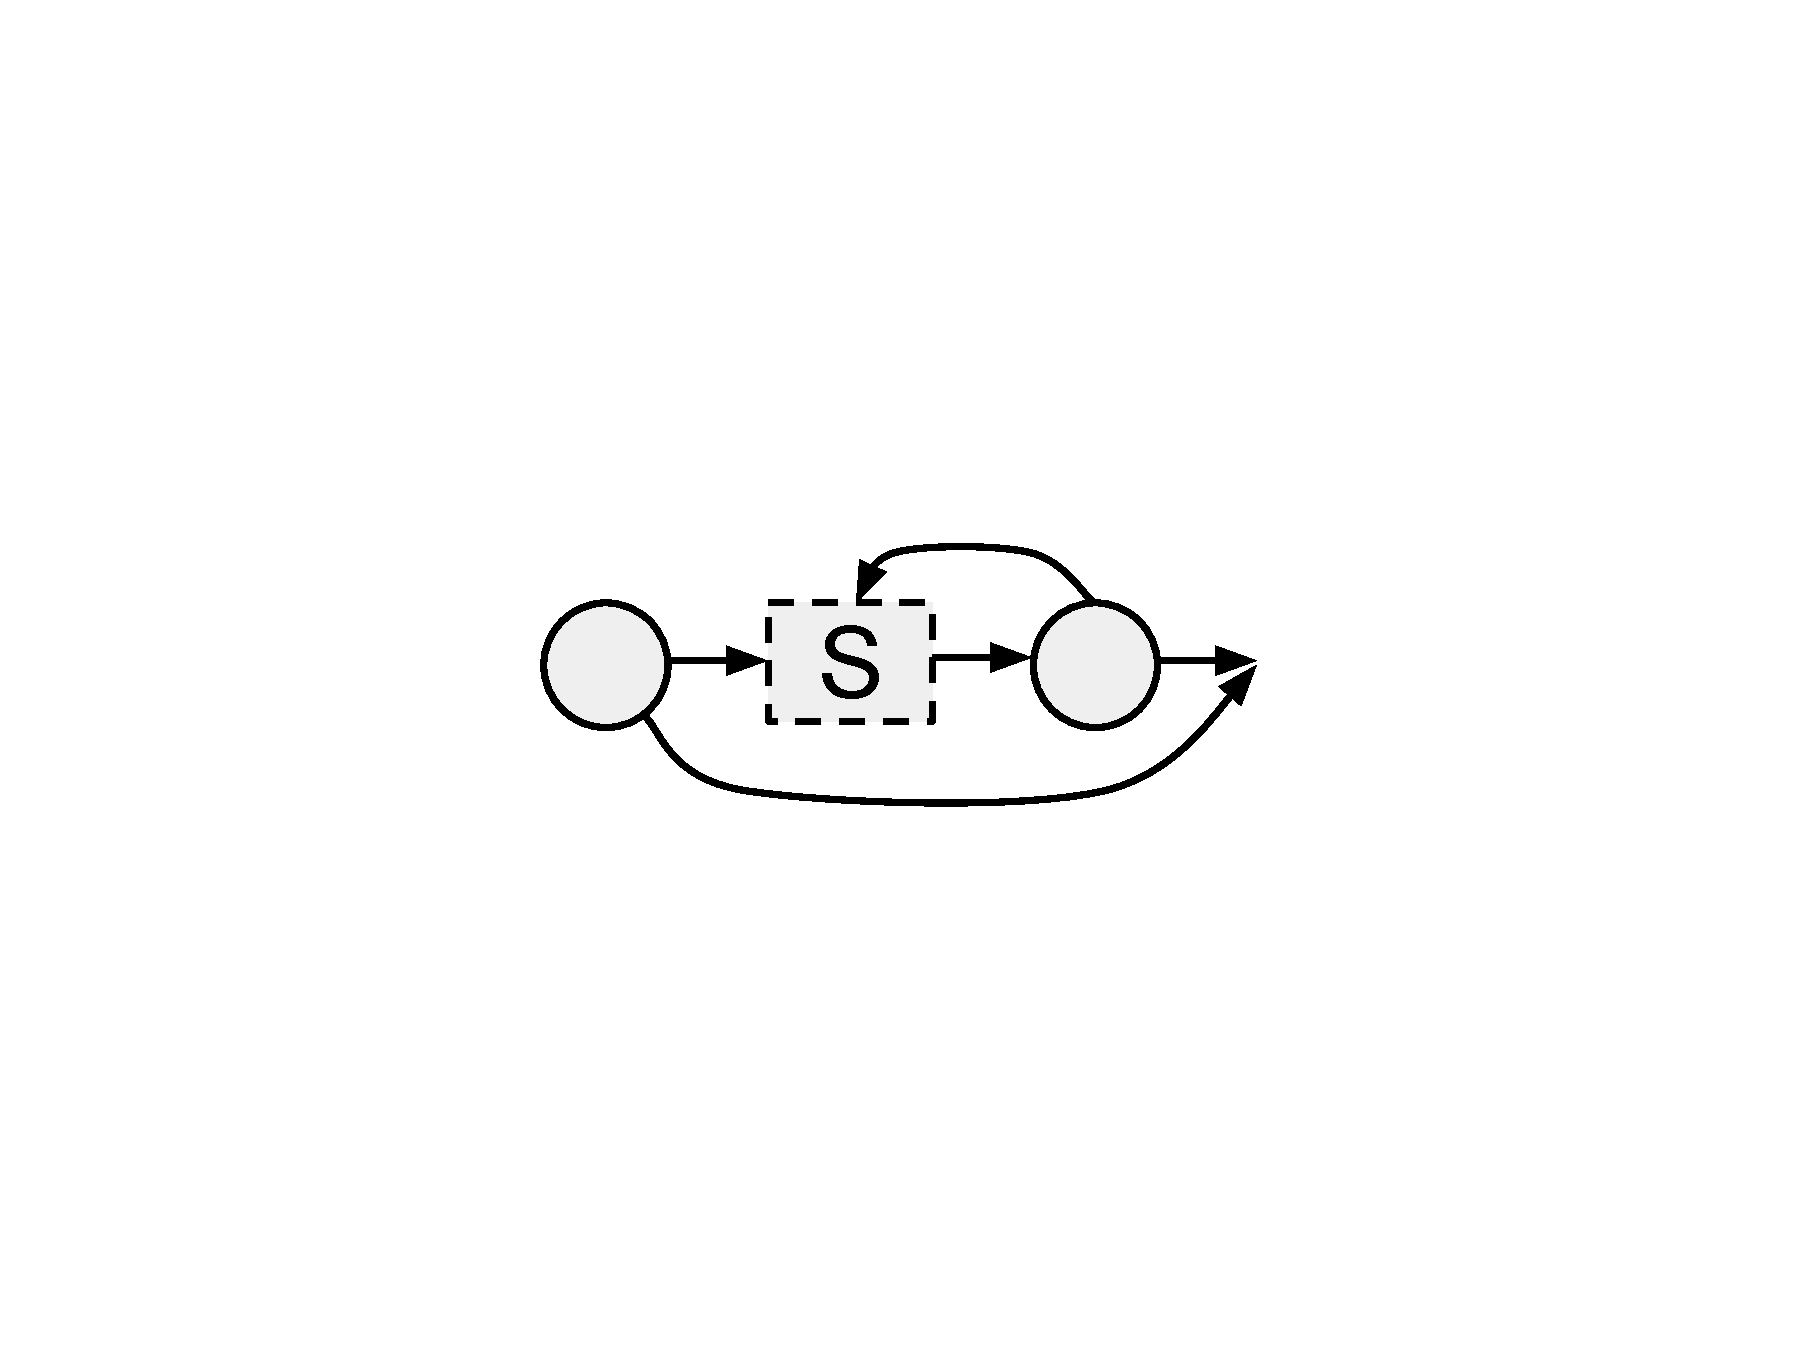
\includegraphics[trim=4in 3.7in 4in 3.5in, scale=0.20]{figures/thompson_kleene.pdf} &
            \texttt{JUMP (+1, <size of S>+2)} \newline
            \texttt{<instructions of S>}  \newline
            \texttt{JUMP (+1, -<size of S>)}
        \\
		\hline
	\end{tabular}
\end{center}
\end{table}

To convert an automaton using these rules, simply traverse the AST in post-order, initially processing all literals and recursively using them as input to the upper nodes. Figure~\ref{fig:exemplo_automato_completo} shows an example of conversion using the expression $(a|a)^+b$.

\begin{figure}[!htbp]
  \centering
  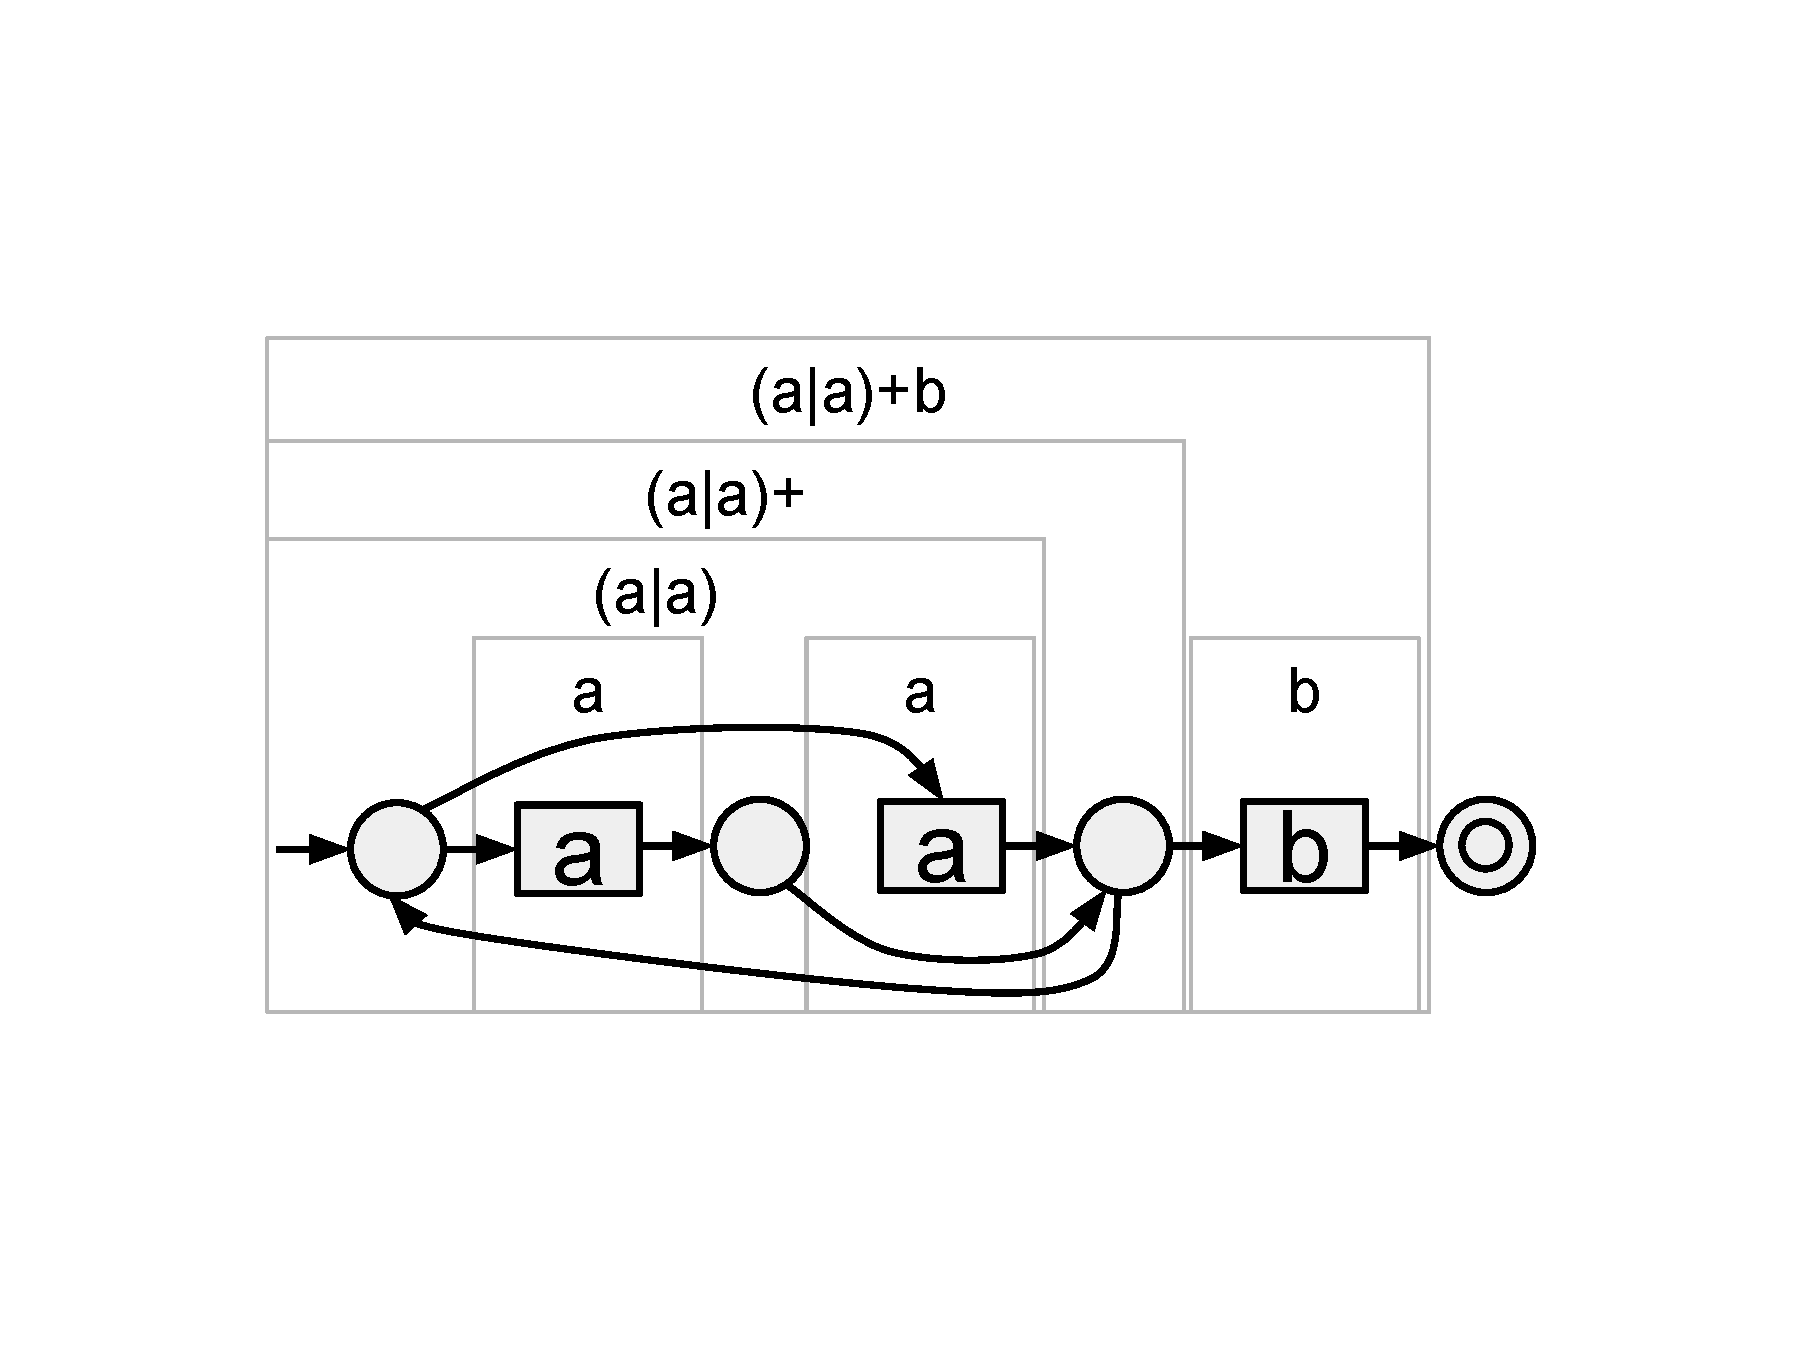
\includegraphics[trim=2in 2in 2in 3in, scale=0.25]{figures/complete_example_automaton.pdf}
  \caption{Example of construction for automaton $(a|a)^+b$}
  \label{fig:exemplo_automato_completo}
\end{figure}

In an optimized implementation, this step can be replaced by machine code generation (as in Thompson's original paper). However, for didactic purposes we describe some useful representations of the generated automaton. 

%~~~~~~~~~~~~~~~~~~~~~~~~~~~~~~~~~~~~~~~~~~~~~~~~~~~~~~~~~~~~~~~~~~~~~~~
\subsection{Simulation}
%~~~~~~~~~~~~~~~~~~~~~~~~~~~~~~~~~~~~~~~~~~~~~~~~~~~~~~~~~~~~~~~~~~~~~~~

Simulating the execution of a non-deterministic automaton using a deterministic machine is a hard problem in itself. There may be an exponential number of possible paths in the automaton \cite{bib:Rabin59}. This is the exact spot where most implementations fail to find a polynomial solution.

But given that we are not interested in all paths, but only if one of them leads to an accept state, there are some easier options to simulate those automata. Some of them are:

\begin{description}
    \item[Backtracking] to try all possible paths, one at a time, rewinding to the last choice in case of failure;
    \item[Backtracking with memoization] same as previous, but memorizing if one state leads to an accept state, given some part of the input;
    \item[Convert to DFA] to eagerly convert the NFA to a deterministic automaton before execution;
    \item[Parallel simulation] to simulate all possible state transitions concurrently, pruning repeated states;
	\item[Lazy DFA conversion] similar to parallel simulation, but memorizing which sets of states have transitions between them, which is the same as lazily converting to a DFA.
\end{description}

The chosen method for this implementation was the \emph{parallel simulation}. It consists, whenever faced with a decision, in choosing both options simultaneously, and keeping parallel executions. 

Initially, it may seem that this leads to a set of up to $2^n$ states running simultaneously, but given that the automaton has a finite number of states, there are at most $m$ possible states running at any time (for each input character). This is so because eventually multiple decisions can collide in the same state, thus eliminating the exponential nature of the evaluation. So, for an input with $n$ characters evaluated against an automaton $m$ states, the worst case time complexity is $O(n \times m)$. 

The goal is that, at runtime, one character will be read at a time. Then, before each run it must evaluate all $\epsilon$ transitions and keeps all flows on hold positioned in {\sc Consume} states.

The main advantage is to have polynomial running time ($O(n \times m)$). Also, it just needs to read the input once and does not require the use of stack. However, it needs additional memory ($O(m)$). And compared to running with a converted DFA it is slower to recognize strings.

%======================================================================================
\section{Implementation}\label{cap:implementation}
%======================================================================================

In this section we will discuss the implementation of the library \emph{Pyrex} (Python Regular Expressions).

The initial goal was to achieve a truly polynomial regular expressions implementation. After that, the implementation was focused on simplicity. We avoided implementation tricks to improve performance at the expense of readability. All choices were made to reduce implementation complexity. Even so, the algorithm used was efficient enough to have better worst-case performance than most implementations.

We chose Python to implement this project. Python is a virtual machine language, like Java. However, its virtual machine does not have the runtime optimizations that most Java implementations have. Also, its dynamic typing sometimes makes it even slower than other static typed languages. Even so, due to the reduced amount of special characters in its syntax, programs written in Python are usually more readable and simpler. 

The entire implementation of Pyrex has 67 lines of code and less than 3KB. This implementation covers regular expression parsing, a rudimentary error handling, automaton construction and simulation.

The project was implemented using only Python 2.7 standard library, but it also works in Python 3.0 and higher.

\subsection{Features}

The features were chosen as the minimum set to make possible to compare Pyrex and other implementations, while being simple enough to be explainable in a few minutes. So, we implemented:

\begin{itemize}
    \item Literals (e.g. $a$)
    \item Sequences (e.g. $ab$)
    \item Options (e.g. $ab|cd$)
    \item Optionals (e.g. $a?$)
    \item Kleene* (e.g. $a^*$)
    \item Kleene+ (e.g. $a^+$)
\end{itemize}

These features are very close to those described by Thompson \cite{bib:Thompson68} and they make it possible to unambiguously represent regular languages.

\subsection{Code structure}

The code is basically divided into two parts: a \emph{parser} and a \emph{matcher}.

The \emph{parser} is responsible for receiving a string with a regular expression, to syntactically parse it and to return an object (the \emph {matcher}) that is able to recognize strings which are part of the regular language defined. 

The \emph {matcher} contains information of the generated automaton and functions that can simulate its execution. It is implemented as a Python class with a \emph{match} method, besides the overloading of the operator \emph{\_\_repr\_\_} of Python, which provides a useful view of the object at debug time. 

To use \emph{Pyrex}, one must compile the automaton using the \emph{rex} function, and then evaluate strings using the \emph{match} method of the \emph {Machine} class. An example can be seen below: 

\begin{verbatim}
import pyrex
machine = pyrex.rex('a(ab)+')
print machine.match('aababxx')
\end{verbatim}

The \emph{match} function return can be either a tuple with two elements (indexes start and end of the match) or a null reference (\emph {None} in Python). In the example, the return would be a tuple $(0,5)$, indicating that the match starts at index 0 of the string and ends at index 4. Notice that the tuple denotes an open interval to the right. 

\subsection{Parsing}

Parsing is done by the function \emph {rex}. It implements a rudimentary recursive descending parser. The EBNF is described below:


\begin{verbatim}
<option>     ::= <sequence> { "|" <sequence> }*
<sequence>   ::= { <repetition> }*
<repetition> ::= <primary> { "*" | "?" | "+" }*
<primary>    ::= "." | <literal> | "(" <option> ")"
\end{verbatim}

It is important to note the detail of the rule \emph {sequence} that allows empty strings. This is a change that allows empty strings as regular expressions (which is useful in some cases). However, this change also allows regular expressions like $a||b$. Which does not constitute an error. The implementation of this rule can be seen below. 

\begin{verbatim}
def sequence():
    e = []
    while tokens and tokens[0] not in '|)':
        e += repetition()
    return e
\end{verbatim}

The implementation is simple, it uses an instance of the  \emph{deque} class as tokens buffer and recursive calls to implement the rules. For each of the four rules defined the EBNF, there is a nested method in \emph {rex} to represent it. 

Error handling is simple but effective. Whenever an unexpected character is encountered in the input, it is reported. One of the mechanisms can be observed in the main parser code below, where after consuming all possible characters, if there are still remaining ones at the entrance, an exception is thrown.

\begin{verbatim}
e = option()
if tokens: 
    raise Exception('Not expected: "{}"'.format(''.join(tokens)))

return Machine(e)
\end{verbatim}

\subsection{Representation}

During the parsing, the regular expression is transformed into a representation of the associated automaton. This automaton is represented as an \emph {array} of objects, where each position of the array represents a state of the automaton. 

As defined in Section~\ref {sec:Notacao} (page~\pageref {sec:Notacao}), the notation used in this automaton provides three types of state: \textsc{Consume} \textsc{Jump} and \textsc{Match}. \textsc{Consume} states are represented by the character they consume. \textsc{Jump} states are represented by a tuple of integers that inform how many states ahead or behind it should `skip'. \textsc{Match} states do not need representation because they always occur at the end of the automaton (according to this notation). 

For example, the automaton 

\begin{figure}[!htbp]
  \centering
  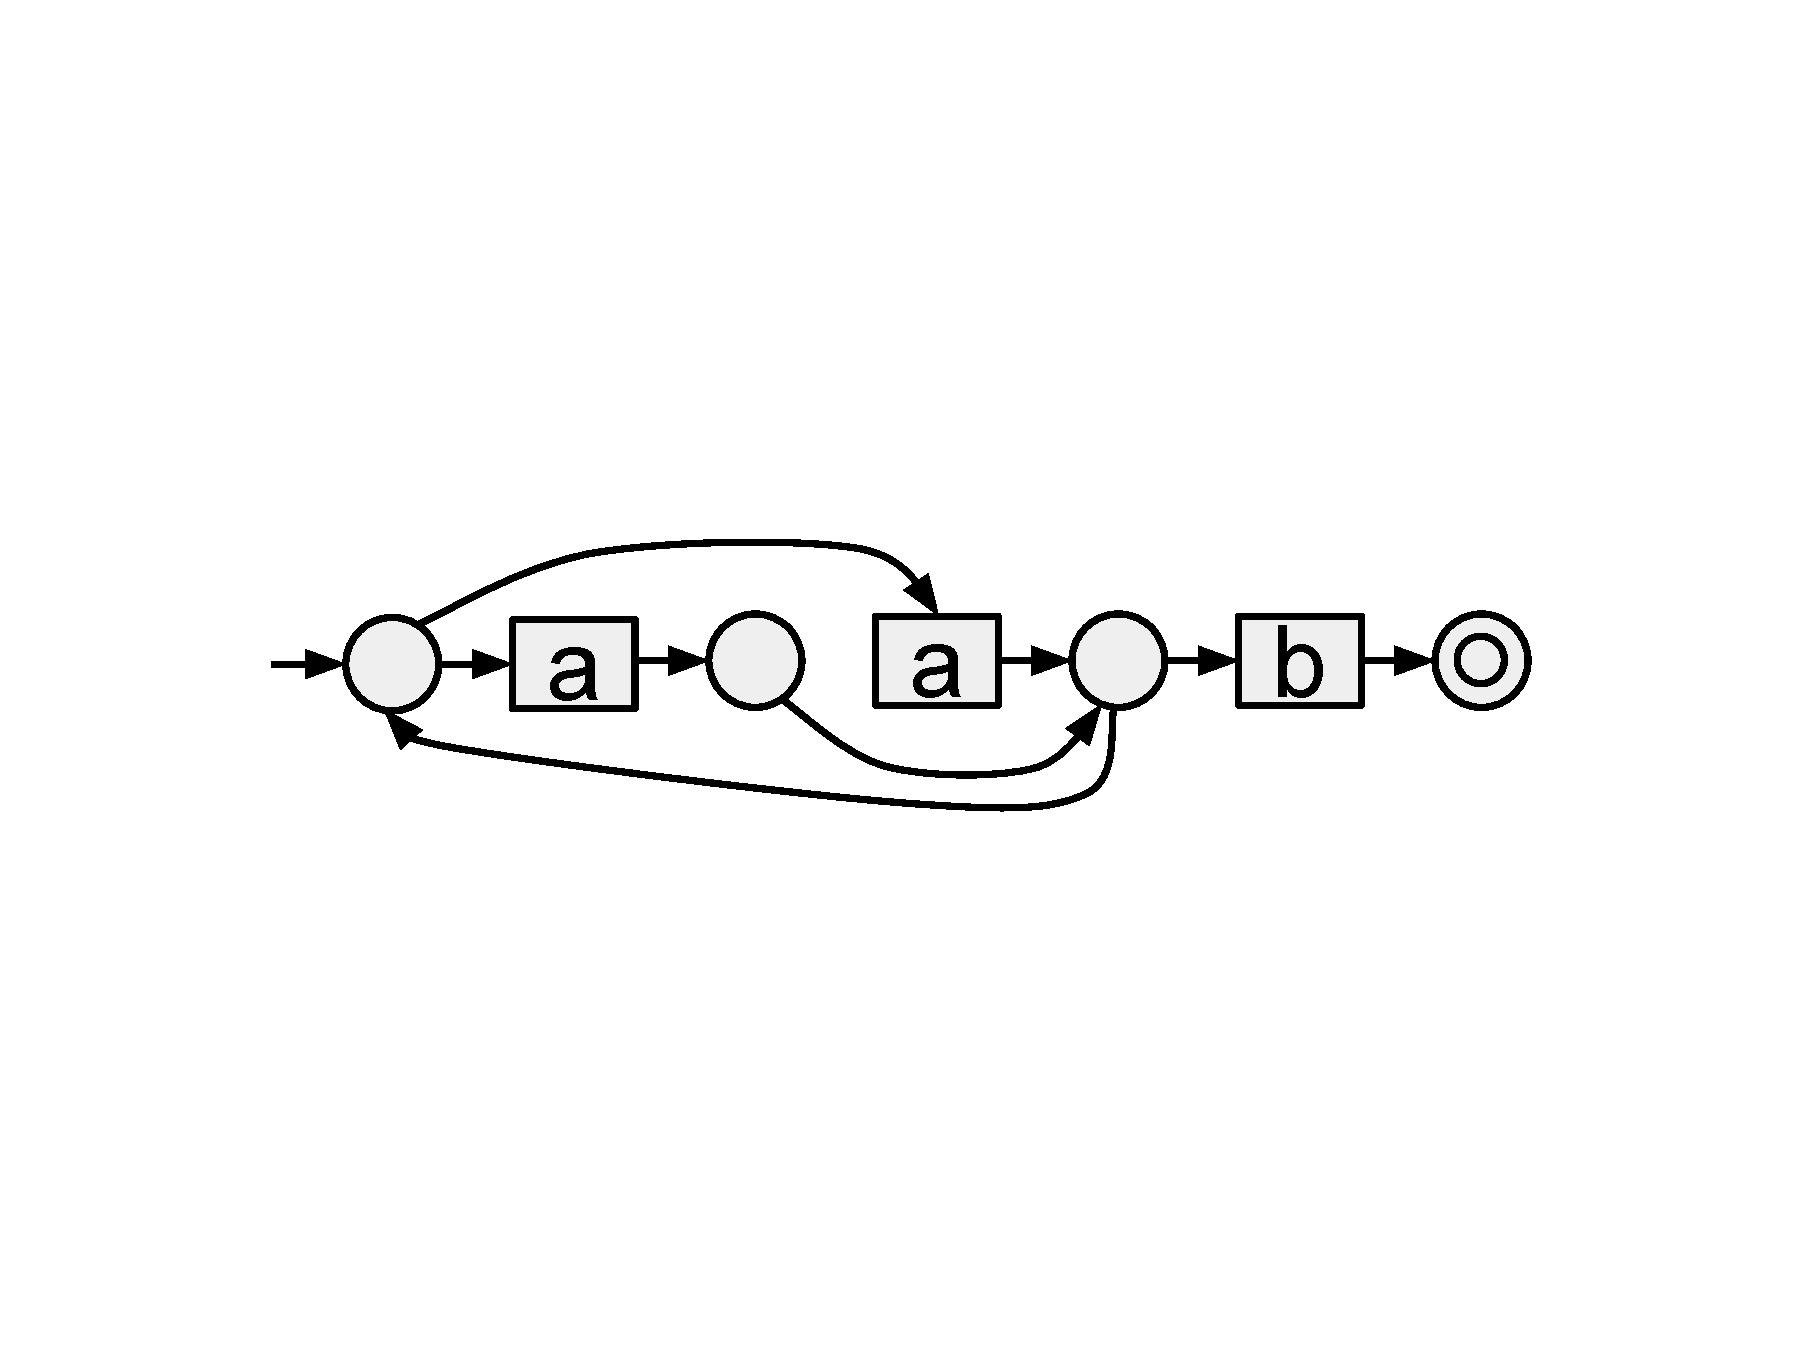
\includegraphics[trim=3.5in 4in 3.5in 4in, scale=0.3]{figures/pure_automaton.pdf}
  \caption{Representation of the automaton as a state diagram}
  \label{fig:exemplo_automato_puro}
\end{figure}

\noindent is equivalent to the array 

\begin{verbatim}
	[(1, 3), 'a', (2,), 'a', (1, -4), 'b']
\end{verbatim}

\noindent which can also be represented as instructions 

\begin{verbatim}
0000: JUMP (1, 3)
0001: CONSUME a
0002: JUMP (2,)
0003: CONSUME a
0004: JUMP (1, -4)
0005: CONSUME b
0006: MATCH!
\end{verbatim}


\subsection{Simulation}

The simulation is performed by the \emph{matcher} and \emph{match} methods of \emph {Machine} class. The difference between them is that the first returns an iterator that assesses the state of execution of the automaton for each input character. The second just returns the result of the match in the end. In the implementation, the  \emph {match} method uses the  \emph {matcher} method, as shown in the snippet below: 

\begin{verbatim}
def match(self, string):
    return reduce(lambda _, s: s[1], self.matcher(string), None)
\end{verbatim}

The method implemented for the simulation of the automaton is the \emph {parallel simulation}. This method was chosen because it combines a polynomial asymptotic complexity with a reasonable ease of implementation. 

As is customary in the implementation of regular expressions, the match is performed in case any substring of the input belongs to the language defined. The parallel simulation method is more advantageous as it requires little change in order to support this mode of execution.

The implementation is based on cycles of use, where a set of initial states simultaneously goes through a transition with the same character $c$ for a set of subsequent states.

In order to represent the states, we use two lists, A and B, which at all times represent respectively the set of states \emph {of consumption}  achieved by the beginning of the evaluation of the current character (A) and the set of states that the evaluation of the current character will reach (B). After the evaluation of each character these lists are reversed.

Each state in these lists comes with the position in the original string where the match began. This information is created when the initial state is placed on the list for each character. It is then copied each time the state is resolved and advances to their successors. In the list, the state is represented by a tuple $ (start, j) $, where $ start$ is the position in the input where the match began and $ j $ is the index of the current state.

It is important to observe that the same state never enters in list B twice in the same cycle of consumption. This check is performed by the array V, which controls the index of the last character where each state joined the list of states. Initially, this list is populated with values  -1. 

As only \textsc{Consume} states enter the lists of states to participate in the consumption cycle (for obvious reasons), all  \textsc{Jump} states must be assessed before the start of the consumption cycle. 

The implementation of the \emph{addnext} method adds states to the following list of consumption (B), recursively solving \textsc{Jump} states in their respective following \textsc{Consume} states. This method also returns the number of times the \textsc{Match} state was reached. 

\begin{verbatim}
def addnext(start, i, j):
    if j==self.n: return 1
    if V[j] == i: return 0
    V[j] = i

    if isinstance(self.states[j], tuple):
        return sum(addnext(start, i, j+k) for k in self.states[j])

    B.append((start, j))
    return 0
\end{verbatim}

Thus, each consumption cycle is characterized by the steps: 

\begin{itemize}
    \item Start new flow in the initial state with the current character. 
    \item Invert lists of \textsc{Consume}, cleaning the list of next (B).
    \item Evaluate the consumption of the current character adding subsequent states in the next list. 
\end{itemize}

The implementation of these steps can be seen below: 

\begin{verbatim}
def key(a): return (a[1]-a[0], -a[0]) if a else (0, 0)

answer = None
for i, c in enumerate(string):
    addnext(i, i, 0)
    yield i, answer, B
    
    A, B = B, A
    del B[:]

    for start, j in A:
        if self.states[j] in (None, c) and addnext(start, i+1, j+1):
            answer = max(answer, (start, i+1), key=key)
    
yield len(string), answer, B
\end{verbatim}

Initially a new flow is added starting at character $i$. Then the \textsc{Consume} lists are reversed. Finally, the \textsc{Consume} states are evaluated against the input, the due states advance, in addition to updating the best response, in case some of these states is a \textsc{Match} state. 

\subsection{\emph{match} Method Return}

To recognize words using regular expressions is a \emph {decision} problem. However, it has proven useful over time to recognize not only strings in regular languages, but also any sub-string belonging to it, then returning their location in the source string.

A regular expression $abcd$ would return a valid match in a string $zzabcdzz$. This behavior allows multiple solutions to be valid. For example, the same expression could find two different results in the word $abcdabcd$. Indeed, many results could overlap. The expression $a^*$, when evaluating the word $aaaa$ can lead to 10 different results. The implementation used greatly influences the choice of which results should be returned. 

The implementation proposed in this project always favors the longest answers. In case of a tie, the favored answer will be the one that starts leftmost in the input. 

This behavior is consistent with the original article by Thompson and, consequently, with implementation of tools such as \emph{sed} and \emph{grep} of the Unix operating system. On the other hand, it differs from other usual implementations based on Perl, which generally return the first answer found by following a greedy order of evaluation \cite{bib:Cox07}. 

An easy way to verify this is to compare the difference of the match expression
$a^*(b|abc)$ against string $abc$. The default implementation of Python returns the string $ab$. The implementation of this project will find the string $abc$. The difference is that Python's implementation attempts to greedly match the longest string with $a^*$, while \emph{Pyrex} can find the longest answer to the entire expression. 

\subsection{Preview}

Drawing on the implementation of the \emph{matcher} method it was possible to build a preview function in text mode, showing the step-by-step execution of the algorithm. It aims to facilitate the understanding of the method. It is a command line tool, also written in Python, that uses the \emph{Pyrex}. 

The previewer can be called with the command \texttt{./view.py (regex) (input)}. For example: 

\begin{verbatim}
./view.py a+b+c+ aabbbcccc
\end{verbatim}

In the example, the execution of the program would show the steps of the match of this regular expression. The automaton generated can be seen in Figure~\ref {fig:view_automaton}. Some steps of the implementation can be seen below: 

\begin{figure}[!htbp]
  \centering
  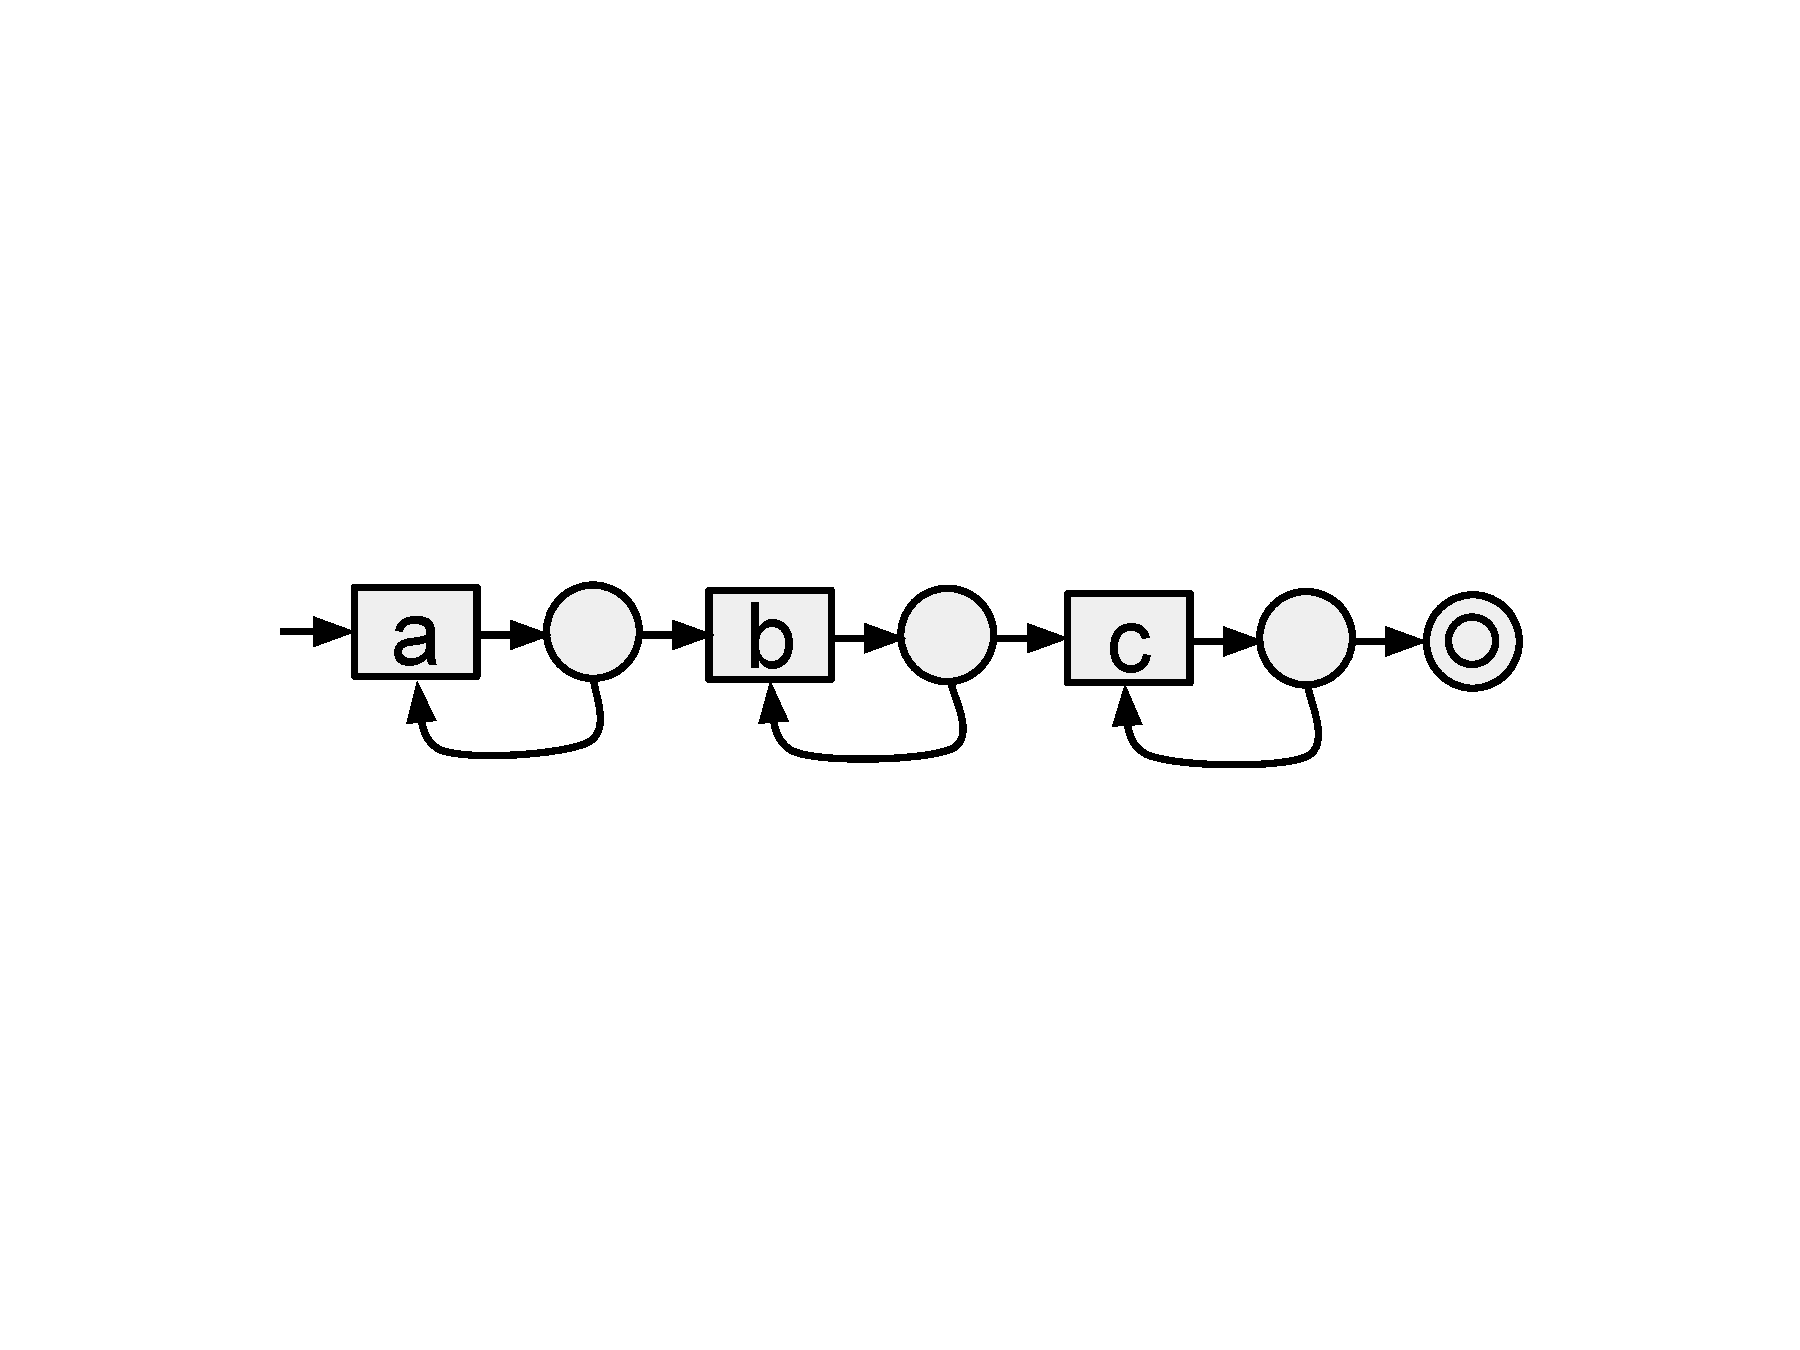
\includegraphics[trim=3.5in 4in 3.5in 4in, scale=0.3]{figures/view_automaton.pdf}
  \caption{Automaton for the expression $a^+b^+c^+$}
  \label{fig:view_automaton}
\end{figure}

\begin{verbatim}
Best answer: <none>
Input: aabbbcccc
          ^ (3)

  3 >0000: CONSUME a
     0001: JUMP (1, -1)
  0 >0002: CONSUME b
     0003: JUMP (1, -1)
  0 >0004: CONSUME c
     0005: JUMP (1, -1)
     0006: MATCH!
\end{verbatim}

This form of display shows the current status of all flows being executed by the automaton. The number displayed next to each statement is the index of the input where that flow started. In the specific example, there are three flows running: 

\begin{itemize}
\item{The one that starts with each character in the string. (3)}
\item{The one that keeps reading characters b from the input, while there still are. (0)}
\item{The one that is ready to read characters c when they start. (0)}
\end{itemize}

\begin{verbatim}
Best answer: aabbbc (0, 6)
Input: aabbbcccc
             ^ (6)

  6 >0000: CONSUME a
     0001: JUMP (1, -1)
     0002: CONSUME b
     0003: JUMP (1, -1)
  0 >0004: CONSUME c
     0005: JUMP (1, -1)
     0006: MATCH!
\end{verbatim}

At this time, there is already a match for the string (since there are already  characters c read). The best match up to this point is shown on the line \emph {Best answer}. This value is updated at every step. In addition, the following states are active:


\begin{itemize}
\item{The one that starts with each character in the string. (6)}
\item{The one that keeps reading c characters at the input while there still are. (0)}
\end{itemize}

The tool uses the matcher method, which returns an iterator that, at each iteration, returns a tuple $(i, answer, state)$, where $i$ is the current index being read at the input, $answer$ is the best response to date and $state$ is the current list of states, which is composed of several tuples $(start, j)$. 

\section{Benchmarks}

Even though the matching of \emph{backreferences} is an NP-complete problem, matching regular expressions itself is not. The main objective of this work is to show that even in cases where expressions could be evaluated in polynomial time, it does not happen in a great part of modern implementations.

In order to demonstrate this point, some tests were made using the same regular expression in various implementations and comparing their execution times considering the growth of the input string. Versions of environments where benchmarks were run are shown in Table~\ref{table:versions}. 

\begin{table}
\begin{center}
	\caption{Versions of the tested implementations}
	\begin{tabular}{ c | c | c }
		\hline 
		{\bf Implementation} & {\bf Environment} & {\bf Original language} \\
		\hline 
		pyrex & Python 2.7.3 & Python \\
		re & Python 2.7.3 & C \\
		Oniguruma & Ruby 1.9.3 & C \\
		java.util.regex & Java 1.6.0\_45 & Java \\
		\hline 
	\end{tabular}
	\label{table:versions}
\end{center}
\end{table}


All graphics are in logarithmic scale to facilitate visualization of the large range of values that each implementation represents. 

\subsection{Benchmark 1: (a?a)+b}

In this test the string $a^n$ was evaluated against the regular expression $(a?a)^+b$. The aim is to show the exponential behavior of implementations based on backtracking. The expression chosen forces the choice for each input character about whether or not to use or not the character $a$ in the expression $a?$. 

Figure~\ref {fig:graph_bench_1} shows the execution time for the different implementations. 

\begin{figure}[!htbp]
\centering
\begin{tikzpicture}[scale=0.6]
	\begin{semilogyaxis}[xlabel=n, ylabel=time (s), legend columns=1, 
	    cycle list name=black white, legend style={legend pos=outer north east, font=\Large}]
	\addplot[mark=triangle*] table[x=n,y=pyrex] {benchmark/bench1.txt};
	\addplot[mark=square*] table[x=n,y=python] {benchmark/bench1.txt};
	\addplot[mark=*] table[x=n,y=ruby] {benchmark/bench1.txt};
	\addplot[mark=x] table[x=n,y=java] {benchmark/bench1.txt};
	\legend{pyrex, python, ruby, java}
	\end{semilogyaxis}
\end{tikzpicture}
\caption{Runtime (in logarithmic scale) to match $a^n$ against $(a?a)^+b$}
\label{fig:graph_bench_1}
\end{figure}

It should be observed that the implementation in Java, which initially has the worst performance, quickly suffers JIT compilation (\emph{Just in Time}), which causes the runtime to drop significantly, while keeping its exponential character. 

\subsection{Benchmark 2: a*b}

In this test, the goal was to demonstrate the high constant of Pyrex implementation in cases where the execution time is linear for all implementations.

Figure~\ref {fig:graph_bench_2} shows the execution time for the different implementations.

\begin{figure}[!htbp]
\centering
\begin{tikzpicture}[scale=0.6]
	\begin{semilogyaxis}[xlabel=n, ylabel=time (s), legend columns=1, 
	    cycle list name=black white, legend style={legend pos=outer north east, font=\Large}]

	\addplot[mark=triangle*] table[x=n,y=pyrex] {benchmark/bench2.txt};
	\addplot[mark=square*] table[x=n,y=python] {benchmark/bench2.txt};
	\addplot[mark=*] table[x=n,y=ruby] {benchmark/bench2.txt};
	\addplot[mark=x] table[x=n,y=java] {benchmark/bench2.txt};
	\legend{pyrex, python, ruby, java}
	\end{semilogyaxis}
\end{tikzpicture}
\caption{Runtime (in logarithmic scale) to match $a^n$ against $a^*b$}
\label{fig:graph_bench_2}
\end{figure}

A clear disadvantage may be observed in implementations in managed code (Pyrex and Java) against other implementations written in C (Ruby and Python) for cases where time complexity is linear.


\subsection{Benchmark 3: a*a*a*a*a*b}

In this test, the goal was to demonstrate how even in cases where implementations based on backtracking do not generate exponential running time, it is still possible to achieve higher execution time than $O(n)$. This expression forces a backtracking for consumption of several repetitions $a^*$. The expected running time of implementations based on backtracking is $O(n^5)$. 

Figure~\ref{fig:graph_bench_3} shows the execution time for the different implementations.

\begin{figure}[!htbp]
\centering
\begin{tikzpicture}[scale=0.6]
	\begin{semilogyaxis}[xlabel=n, ylabel=time (s), legend columns=1, 
	    cycle list name=black white, legend style={legend pos=outer north east, font=\Large}]
	\addplot[mark=triangle*] table[x=n,y=pyrex] {benchmark/bench3.txt};
	\addplot[mark=square*] table[x=n,y=python] {benchmark/bench3.txt};
	\addplot[mark=*] table[x=n,y=ruby] {benchmark/bench3.txt};
	\addplot[mark=x] table[x=n,y=java] {benchmark/bench3.txt};
	\legend{pyrex, python, ruby, java}
	\end{semilogyaxis}
\end{tikzpicture}
\caption{Runtime (in logarithmic scale) to match $a^n$ against $a*a*a*a*a*b$}
\label{fig:graph_bench_3}
\end{figure}

This result also shows how certain static optimizations allow the implementation of Ruby to keep its running time linear while the Python implementation which is also written in C, has a time complexity greater than that of \emph{Pyrex}.


\section{Conclusion}

The main contribution of this work was a didactic implementation of regular expressions using the Thompson Construction Algorithm. A simple method was used to represent the states of non-deterministic finite automata as instructions of an abstract machine that can be deployed on any platform. The implementation was done in Python for simplicity and didactic purposes.

The results were quite satisfactory, showing that it is possible to implement regular expressions with polynomial algorithms. The implementation, though not the most efficient for trivial cases, proved to be very useful to demonstrate the didactically well-established theory of regular expressions. 

The inability of implementations in languages like Python, Ruby, and Java to recognize them in polynomial time (in the worst case) was also demonstrated, even for some expressions without \emph{backreferences}. 

These results confirm the need for parsimony when using regular expressions, especially in software that share hardware resources among multiple users, e.g. websites and other network services. 

\begin{thebibliography}{10}
\providecommand{\url}[1]{\texttt{#1}}
\providecommand{\urlprefix}{URL }

\bibitem{bib:Campeanu07}
C{\^a}mpeanu, C. and Santean, N.: On pattern expression languages. 
  Proceedings AutoMathA (2007)

\bibitem{bib:Chomsky57}
Chomsky, N.: I.r.e. transactions on information theory. Bulletin of
  Mathematical Biophysics  2,  113--124 (1957)

\bibitem{bib:Chomsky58}
Chomsky, N., Miller, G.A.: Finite state languages. Information and control
  1(2),  91--112 (1958)

\bibitem{bib:Cook71}
Cook, S.A.: The complexity of theorem-proving procedures. In: Proceedings of
  the third annual ACM symposium on Theory of computing. pp. 151--158. ACM
  (1971)

\bibitem{bib:Cox07}
Cox, R.: Regular expression matching can be simple and fast (2007),
  \url{http://swtch.com/\textasciitilde{}rsc/regexp/regexp1.html}

\bibitem{bib:Karp72}
Karp, R.M.: Reducibility among combinatorial problems. Springer (1972)

\bibitem{bib:Kirrage13}
Kirrage, J., Rathnayake, A., Thielecke, H.: Static analysis for regular
  expression denial-of-service attacks. Springer LNCS (7873) (2013)

\bibitem{bib:Kleene56}
Kleene, S.C.: Representation of events in nerve nets and finite automata. In
  Automata Studies, Ann. Math. Stud. (34),  3--41 (1956)

\bibitem{bib:Levin73}
Levin, L.A.: Universal sorting problems. Problems of Information Transmission
  9(3),  265--266 (1973)

\bibitem{bib:McCulloch43}
Mcculloch, W., Pitts, W.: A logical calculus of ideas immanent in nervous
  activity. Bulletin of Mathematical Biophysics  5,  127--147 (1943)

\bibitem{bib:Nikita12}
Popov, N.: The true power of regular expressions (2012),
  \url{http://nikic.github.io/2012/06/15/The-true-power-of-regular-expressions.html}

\bibitem{bib:Rabin59}
Rabin, M.O., Scott, D.: Finite automata and their decision problems. IBM
  journal of research and development  3(2),  114--125 (1959)

\bibitem{bib:Ruohonen09}
Ruohonen, K.: Formal languages. lecture notes for the TUT course "Formaalit
  kielet"  (2009)

\bibitem{bib:Thompson68}
Thompson, K.: Regular expression search algorithm. Communications of the ACM
  11(6),  419--422 (jun 1968)

\bibitem{bib:Veldhuizen03}
Veldhuizen, T.L.: C++ templates are turing complete. Available at citeseer.
  ist. psu. edu/581150. html  (2003)

\bibitem{bib:Weidman10}
Weidman, A.: Regular expression denial of service - redos (2010),
  \url{https://www.owasp.org/index.php/Regular\_expression\_Denial\_of\_Service\_-\_ReDoS}

\end{thebibliography}

\end{document}

